%  template.tex for Biometrics papers
%
%  This file provides a template for Biometrics authors.  Use this
%  template as the starting point for creating your manuscript document.
%  See the file biomsample.tex for an example of a full-blown manuscript.

%  ALWAYS USE THE referee OPTION WITH PAPERS SUBMITTED TO BIOMETRICS!!!
%  You can see what your paper would look like typeset by removing
%  the referee option.  Because the typeset version will be in two
%  columns, however, some of your equations may be too long. DO NOT
%  use the \longequation option discussed in the user guide!!!  This option
%  is reserved ONLY for equations that are impossible to split across 
%  multiple lines; e.g., a very wide matrix.  Instead, type your equations 
%  so that they stay in one column and are split across several lines, 
%  as are almost all equations in the journal.  Use a recent version of the
%  journal as a guide. 
%  
%\documentclass[useAMS,usenatbib]{biom}
%\documentclass[useAMS,usenatbib,referee]{biom}
\documentclass[12pt,letter]{article}\usepackage[]{graphicx}\usepackage[]{color}
%
%  If your system does not have the AMS fonts version 2.0 installed, then
%  remove the useAMS option.
%
%  useAMS allows you to obtain upright Greek characters.
%  e.g. \umu, \upi etc.  See the section on "Upright Greek characters" in
%  this guide for further information.
%
%  If you are using AMS 2.0 fonts, bold math letters/symbols are available
%  at a larger range of sizes for NFSS release 1 and 2 (using \boldmath or
%  preferably \bmath).
% 
%  Other options are described in the user guide. Here are a few:
% 
%  -  If you use Patrick Daly's natbib  to cross-reference your 
%     bibliography entries, use the usenatbib option
%
%  -  If you use \includegraphics (graphicx package) for importing graphics
%     into your figures, use the usegraphicx option
% 
%  If you wish to typeset the paper in Times font (if you do not have the
%  PostScript Type 1 Computer Modern fonts you will need to do this to get
%  smoother fonts in a PDF file) then uncomment the next line
%  \usepackage{Times}

%%%%% PLACE YOUR OWN MACROS HERE %%%%%

\def\bSig\mathbf{\Sigma}
\newcommand{\VS}{V\&S}
\newcommand{\tr}{\mbox{tr}}

%  The rotating package allows you to have tables displayed in landscape
%  mode.  The rotating package is NOT included in this distribution, but
%  can be obtained from the CTAN archive.  USE OF LANDSCAPE TABLES IS
%  STRONGLY DISCOURAGED -- create landscape tables only as a last resort if
%  you see no other way to display the information.  If you do do this,
%  then you need the following command.

\usepackage[figuresright]{rotating}

%########################################################################################
%            						PACKAGES
%########################################################################################

\usepackage{authblk} % for author affiliations
\usepackage{float} % for H in figures and tables
\usepackage{amsmath,amssymb,bbm,mathrsfs,mathtools,xfrac} %math stuff
%\usepackage{amsthm}
%\usepackage{cleveref}
%\newcommand{\crefrangeconjunction}{--}
%\usepackage[nomarkers,figuresonly]{endfloat}

\usepackage[sort]{natbib}   % bibliography omit 'round' option if you prefer square brackets
\usepackage{placeins} % for \FloatBarrier
\usepackage[pagebackref=false,bookmarks]{hyperref}
\hypersetup{
	unicode=false,
	pdftoolbar=true,
	pdfmenubar=true,
	pdffitwindow=false,     % window fit to page when opened
	pdfstartview={FitH},    % fits the width of the page to the window
	pdftitle={Sparse Additive Interaction Learning},    % title
	pdfauthor={Sahir Rai Bhatnagar},     % author
	pdfsubject={sail manuscript},   % subject of the document
	pdfcreator={Sahir Rai Bhatnagar},   % creator of the document
	pdfproducer={Sahir Rai Bhatnagar}, % producer of the document
	pdfkeywords={}, % list of keywords
	pdfnewwindow=true,      % links in new window
	colorlinks=true,       % false: boxed links; true: colored links
	linkcolor=red,          % color of internal links (change box color with linkbordercolor)
	citecolor=blue,        % color of links to bibliography
	filecolor=black,      % color of file links
	urlcolor=blue           % color of external links
}
\usepackage[utf8]{inputenc} % for french accents
\usepackage[T1]{fontenc} % for french accents
\usepackage{ctable} % load after tikz. used for tables
\usepackage{pifont}% http://ctan.org/pkg/pifont
\newcommand{\cmark}{\ding{51}}%
\newcommand{\xmark}{\ding{55}}%
\def\widebar#1{\overline{#1}}
\usepackage{array}
\newcolumntype{L}{>{\centering\arraybackslash}m{3cm}} % used for text wrapping in ctable
\usepackage{color, colortbl, xcolor, comment}
\usepackage{subfig}
%\usepackage{tcolorbox} % for box around text
%\usepackage[ruled,vlined,linesnumbered,noresetcount]{algorithm2e}
%\usepackage[ruled,vlined,noresetcount]{algorithm2e}
\usepackage{algorithm}
\usepackage{chngcntr} % for figure labels in appendix
%\usepackage[ruled,vlined,noresetcount]{algorithm2e}
\usepackage[noend]{algpseudocode}
\algrenewcommand\textproc{}% Used to be \textsc
\algdef{SE}[SUBALG]{Indent}{EndIndent}{}{\algorithmicend\ }%
\algtext*{Indent}
\algtext*{EndIndent}
%\usepackage[american]{babel}
%\let\tnote\relax

%\usepackage{csquotes}

\usepackage{pdflscape}

%\usepackage[style=apa,sortcites=true,sorting=nyt,backend=biber]{biblatex}
%\usepackage{epstopdf}

%\usepackage{tabulary}
%\usepackage{siunitx}
%\sisetup{output-exponent-marker=\ensuremath{\mathrm{e}}}
%\AtBeginEnvironment{tabulary}{\onehalfspacing}
%\usepackage{multirow}
%\usepackage{ctable} % NEED TO LOAD CTABLE AFTER TIKZ FOR SOME REASON
%\usepackage{array}
%\newcolumntype{L}{>{\centering\arraybackslash}m{3cm}} % used for text wrapping in ctable
%\usepackage{enumitem}
% These packages are all incorporated in the memoir class to one degree or another...


%########################################################################################
%            						CUSTOM COMMANDS
%########################################################################################

%\newtheorem{theorem}{Theorem}
%\newtheorem{proposition}{Proposition}
%\newtheorem{lemma}{Lemma}
\newcommand{\sgn}{\operatorname{sgn}}
\newcommand{\Op}{O_{P}}
\newcommand{\op}{o_{P}}
\newcommand{\ddd}{,\ldots,}
%\global\long\def\ddd{,\ldots,}
\newcommand{\sail}{\texttt{sail}}
\newcommand{\tm}[1]{\textrm{{#1}}}
\newcommand{\bx}{\textbf{\emph{x}}}
\newcommand{\by}{\textbf{\emph{y}}}
\newcommand{\bX}{\textbf{\emph{X}}}
\newcommand{\bW}{\textbf{\emph{W}}}
\newcommand{\bY}{\textbf{\emph{Y}}}
\newcommand{\bD}{\textbf{\text{D}}}
\newcommand{\bXtilde}{\widetilde{\bX}}
\newcommand{\bYtilde}{\widetilde{\bY}}
\newcommand{\bDtilde}{\widetilde{\bD}}
\newcommand{\Xtilde}{\widetilde{X}}
\newcommand{\Ytilde}{\widetilde{Y}}
\newcommand{\Dtilde}{\widetilde{D}}
\newcommand{\bu}{\textbf{u}}
\newcommand{\bU}{\textbf{\emph{U}}}
\newcommand{\bV}{\textbf{\emph{V}}}
\newcommand{\bE}{\textbf{\emph{E}}}
\newcommand{\bb}{\textbf{\emph{b}}}
\newcommand{\bI}{\textbf{\emph{I}}}
\newcommand{\be}{\boldsymbol{\varepsilon}}
\newcommand{\bSigma}{\boldsymbol{\Sigma}}
\newcommand{\bLambda}{\boldsymbol{\Lambda}}
\newcommand{\bTheta}{\boldsymbol{\Theta}}
\newcommand{\balpha}{\boldsymbol{\alpha}}
\newcommand{\btau}{\boldsymbol{\tau}}
\newcommand{\bgamma}{\boldsymbol{\gamma}}
%\newcommand{\ltwonorm}[1]{\lVert #1 \rVert}
\newcommand{\mb}[1]{\mathbf{#1}}
\newcommand{\mc}[2]{\multicolumn{#1}{c}{#2}}
\newcommand{\mcl}[2]{\multicolumn{#1}{l}{#2}}
\definecolor{Gray}{gray}{0.9}
\newcommand {\bs}{\boldsymbol}
%\newcommand{\norm}[1]{\left\Vert #1 \right\Vert}
\newcommand{\xf}{\mathcal{X}}
\newcommand{\pfrac}[2]{\left( \frac{#1}{#2}\right)}
\newcommand{\e}{{\mathsf E}}
\newcommand{\bt}{\boldsymbol{\theta}}
\newcommand{\bmu}{\boldsymbol{\mu}}
\newcommand{\bbeta}{\boldsymbol{\beta}}
\newcommand{\btheta}{\boldsymbol{\theta}}
\newcommand{\bPhi}{\boldsymbol{\Phi}}
\newcommand{\bPsi}{\boldsymbol{\Psi}}
\DeclareMathOperator*{\argmin}{arg\,min}
\DeclareMathOperator*{\argmax}{arg\,max}
\DeclareMathOperator{\diag}{diag} % operator and subscript

\DeclarePairedDelimiter\abs{\lvert}{\rvert}%
\DeclarePairedDelimiter\norm{\lVert}{\rVert}%

\global\long\def\ddd{,\ldots,}


\newcommand{\bthetastar}{\boldsymbol{\theta}^{*}}
\newcommand{\bThetastar}{\boldsymbol{\Theta}^{*}}
\newcommand{\bdelta}{\boldsymbol{\delta}}
\newcommand{\A}{\mathcal{A}}
\newcommand{\mH}{\mathcal{H}}

% Swap the definition of \abs* and \norm*, so that \abs
% and \norm resizes the size of the brackets, and the
% starred version does not.
\makeatletter
\let\oldabs\abs
\def\abs{\@ifstar{\oldabs}{\oldabs*}}
%
\let\oldnorm\norm
\def\norm{\@ifstar{\oldnorm}{\oldnorm*}}
\makeatother

%########################################################################################
%            						FANCY HEADER STUFF
%########################################################################################
\usepackage{lastpage}
\usepackage{fancyhdr}
\cfoot{\thepage}
\lhead[\leftmark]{}
\rhead[]{\leftmark}
\makeatletter
\makeatother
%\lfoot{} \cfoot{ } \rfoot{{\small{\em Page \thepage \ of \pageref{LastPage}}}}
\lfoot{} \cfoot{ } \rfoot{{\small{\em Page \thepage}}}

%########################################################################################
%            						SPACING
%########################################################################################

\usepackage[parfill]{parskip} % Activate to begin paragraphs with an empty line rather than an indent
%\usepackage[left=.1in,right=.1in,top=.1in,bottom=.1in]{geometry}
\usepackage[margin=1in]{geometry}
\usepackage{setspace}
\doublespacing



%########################################################################################
%            						TITLE and AUTHORS
%########################################################################################

\title{A Sparse Additive Model for High-Dimensional Interactions with an Exposure Variable\\Supplemental Materials}
%\author{SRB}

%David L Olds Department of Pediatrics, University of Colorado School of Medicine, Denver David.Olds@ucdenver.edu

%Michael S. Kobor Department of Medical Genetics, University of British Columbia msk@cmmt.ubc.ca

%Michael J. Meaney, Singapore Institute for Clinical Sciences, Singapore; McGill University, michael.meaney@mcgill.ca

\author[1,2]{Sahir R Bhatnagar}
\author[3,4]{Tianyuan Lu}
\author[5]{Amanda Lovato}
\author[6]{David L Olds}
\author[7]{Michael S Kobor}
\author[8]{Michael J Meaney}
\author[9]{Kieran O'Donnell}
\author[10]{Yi Yang}
\author[1,3,5]{\mbox{Celia MT Greenwood}}

\affil[1]{Department of Epidemiology, Biostatistics and Occupational Health, McGill University}
\affil[2]{Department of Diagnostic Radiology, McGill University}
\affil[3]{Quantitative Life Sciences, McGill University}
\affil[4]{Lady Davis Institute, Jewish General Hospital, Montr\'{e}al, QC}
\affil[5]{Statistics Canada, Ottawa, ON}
\affil[6]{Department of Pediatrics, University of Colorado School of Medicine, Denver}
\affil[7]{Department of Medical Genetics, University of British Columbia, BC}
\affil[8]{Singapore Institute for Clinical Sciences, Singapore; McGill University}
\affil[9]{Department of Psychiatry, McGill University}
\affil[10]{Department of Mathematics and Statistics, McGill University}
\affil[11]{Departments of Oncology and Human Genetics, McGill University}



\begin{document}
		
	\maketitle

	\tableofcontents

\section{Proofs} \label{ap:proofs}

\subsection{Regularity Conditions}


\begin{description}
	\item [{(C1)}] The observation $\{\mathbf{V}_{i}:i=1\ddd n\}$ are independent
	and identically distributed with a probability density $f(\mathbf{V},\boldsymbol{\Phi})$,
	which has a common support. We assume the density $f$ satisfies the
	following equations:
	\[
	E_{\boldsymbol{\Phi}}\left[\nabla_{\boldsymbol{\phi}_{j}}\log f\left(\boldsymbol{V},\boldsymbol{\Phi}\right)\right]=\mathbf{0}\quad\text{for }j=1\ddd2p+1.
	\]
	and 
	\begin{align*}
	\mathbf{I}_{j_{1}k_{1}j_{2}k_{2}}(\boldsymbol{\Phi}) & =E_{\boldsymbol{\Phi}}\left[\frac{\partial}{\partial\phi_{j_{1}k_{1}}}\log f(V,\boldsymbol{\Phi})\cdot\frac{\partial}{\partial\phi_{j_{2}k_{2}}}\log f(V,\boldsymbol{\Phi})\right]\\
	& =E_{\boldsymbol{\Phi}}\left[-\frac{\partial^{2}}{\partial\phi_{j_{1}k_{1}}\phi_{j_{2}k_{2}}}\log f(V,\boldsymbol{\Phi})\right],
	\end{align*}
	for any $j_{1},j_{2}=1\ddd2p+1$, and $k_{1}=1\ddd p_{j1}$, $k_{2}=1\ddd p_{j2}$,
	where $j_{1},j_{2}$ are the index of group, $k_{1},k_{2}$ be the
	index of elements within the corresponding group, $p_{j_{1}},p_{j_{2}}$
	are the group size of $j_{1},j_{2}$ respectively.
	\item [{(C2)}] The Fisher information matrix 
	\[
	\mathbf{I}\left(\boldsymbol{\Phi}\right)=E\left[\left(\frac{\partial}{\partial\boldsymbol{\Phi}}\log f(V,\boldsymbol{\Phi})\right)\left(\frac{\partial}{\partial\boldsymbol{\Phi}}\log f(V,\boldsymbol{\Phi})\right)^{\top}\right]
	\]
	is finite and positive definite at $\boldsymbol{\Phi}=\boldsymbol{\Phi}^{*}$.
	\item [{(C3)}] There exists an open set $\omega$ of $\Omega$ that contains
	the true parameter point $\boldsymbol{\Phi}^{*}$ such that for almost
	all $\mathbf{V}$ the density $f(\mathbf{V},\boldsymbol{\Phi})$ admits
	all third derivatives $\frac{\partial^{3}f(\mathbf{V},\boldsymbol{\Phi})}{\partial\phi_{j_{1}k_{1}}\partial\phi_{j_{2}k_{2}}\partial\phi_{j_{3}k_{3}}}$
	for all $\boldsymbol{\Phi}$ in $\omega$ and any $j_{1},j_{2},j_{3}=1\ddd2p+1$,
	and $k_{1}=1\ddd p_{j1}$, $k_{2}=1\ddd p_{j2}$ and $k_{3}=1\ddd p_{j3}$.
	Furthermore, there exist functions $M_{j_{1}k_{1}j_{2}k_{2}j_{3}k_{3}}$
	such that
	\[
	\left|\frac{\partial^{3}}{\partial\phi_{j_{1}k_{1}}\partial\phi_{j_{2}k_{2}}\partial\phi_{j_{3}k_{3}}}\log f(\mathbf{V},\boldsymbol{\Phi})\right|\leq M_{j_{1}k_{1}j_{2}k_{2}j_{3}k_{3}}(\mathbf{V})\quad\text{for all }\boldsymbol{\Phi}\in\omega,
	\]
	and $m_{j_{1}k_{1}j_{2}k_{2}j_{3}k_{3}}=E_{\boldsymbol{\Phi}^{*}}[M_{j_{1}k_{1}j_{2}k_{2}j_{3}k_{3}}(\mathbf{V})]<\infty$.
\end{description}

\subsection{Lemma 1 proof}

{\normalsize{}Let $\eta_{n}=\frac{1}{\sqrt{n}}+a_{n}$ and $\{\boldsymbol{\Phi}^{*}+\eta_{n}\boldsymbol{\delta}:\|\boldsymbol{\delta}\|_{2}\leq C\}$
	be the ball around $\boldsymbol{\Phi}^{*}$ for $\boldsymbol{\delta}\in\mathbb{R}^{d}$,
	where $d$ is the dimension of the design matrix and $C$ is some
	constant. Under the regularity assumptions, we show that there exists
	a local minimizer $\widehat{\boldsymbol{\Phi}}_{n}$ of $Q_{n}(\boldsymbol{\Phi})$
	such that $\|\widehat{\boldsymbol{\Phi}}_{n}-\boldsymbol{\Phi}^{*}\|_{2}=O_{p}(\frac{1}{\sqrt{n}})$.
	For this proof, we adopt the approaches outlined in~\citep{fan2001variable,choi2010variable,nardi2008asymptotic,wang2007regression}
	and extend it to our situation. Let $\eta_{n}=\frac{1}{\sqrt{n}}+a_{n}$
	and $\{\boldsymbol{\Phi}^{*}+\eta_{n}\boldsymbol{\delta}:\|\boldsymbol{\delta}\|_{2}\leq C\}$
	be the ball around $\boldsymbol{\Phi}^{*}$ for $\boldsymbol{\delta}=(\mathbf{u}_{1}^{\top},\mathbf{u}_{2}^{\top},\ddd\mathbf{u}_{p+1}^{\top},\mathbf{u}_{p+2}^{\top},\ldots,\mathbf{u}_{2p+1}^{\top})^{\top}\in\mathbb{R}^{d}$,
	where $d$ is the dimension of the design matrix and $C$ is some
	constant. The objective function is given by 
	\[
	Q_{n}(\boldsymbol{\Phi})=-L_{n}(\boldsymbol{\Phi})+n\lambda_{m}\sum_{m=1}^{2p+1}\left\Vert \boldsymbol{\phi}_{m}\right\Vert _{2},
	\]
	Define
	\[
	D_{n}(\boldsymbol{\delta})\equiv Q_{n}(\boldsymbol{\Phi}^{*}+\eta_{n}\bdelta)-Q_{n}(\boldsymbol{\Phi}^{*}).
	\]
	Then for $\bdelta$ that satisfies $\|\bdelta\|_{2}=C$, we have
	\begin{align}
	D_{n}(\bdelta) & =-L_{n}(\boldsymbol{\Phi}^{*}+\eta_{n}\bdelta)+L_{n}(\boldsymbol{\Phi}^{*})+n\sum_{m=1}^{2p+1}\lambda_{m}(\|\btheta_{m}^{*}+\eta_{n}\mathbf{u}_{m}\|_{2}-\|\btheta_{m}^{*}\|_{2})\nonumber \\
	& \overset{(a)}{\geq}-L_{n}(\boldsymbol{\Phi}^{*}+\eta_{n}\bdelta)+L_{n}(\boldsymbol{\Phi}^{*})+n\sum_{m\in\mathcal{A}_{1}}\lambda_{m}^{\theta}(\|\btheta_{m}^{*}+\eta_{n}\mathbf{u}_{m}\|_{2}-\|\btheta_{m}^{*}\|_{2})\nonumber \\
	& \quad+n\sum_{m\in\mathcal{A}_{2}}\lambda_{m}^{\theta}(\|\btheta_{m}^{*}+\eta_{n}\mathbf{u}_{m}\|_{2}-\|\btheta_{m}^{*}\|_{2})\nonumber \\
	& \overset{(b)}{\geq}-L_{n}(\boldsymbol{\Phi}^{*}+\eta_{n}\bdelta)+L_{n}(\boldsymbol{\Phi}^{*})-n\eta_{n}\sum_{m\in\mathcal{A}_{1}}\lambda_{m}\|\mathbf{u}_{m}\|_{2}-n\eta_{n}\sum_{m\in\mathcal{A}_{2}}\lambda_{m}\|\mathbf{u}_{m}\|_{2}\nonumber \\
	& \overset{(c)}{\geq}-L_{n}(\boldsymbol{\Phi}^{*}+\eta_{n}\bdelta)+L_{n}(\boldsymbol{\Phi}^{*})-n\eta_{n}^{2}\sum_{m\in\mathcal{A}_{1}}\|\mathbf{u}_{m}\|_{2}-n\eta_{n}^{2}\sum_{m\in\mathcal{A}_{2}}\|\mathbf{u}_{m}\|_{2}\nonumber \\
	& \overset{}{\geq}-L_{n}(\boldsymbol{\Phi}^{*}+\eta_{n}\bdelta)+L_{n}(\boldsymbol{\Phi}^{*})-n\eta_{n}^{2}(|\A_{1}|+|\A_{2}|)C\nonumber \\
	%
	& \overset{(d)}{=}-[\nabla L_{n}(\boldsymbol{\Phi}^{*})]^{\top}(\eta_{n}\bdelta)-\frac{1}{2}(\eta_{n}\bdelta)^{\top}[\nabla^{2}L_{n}(\boldsymbol{\Phi}^{*})](\eta_{n}\bdelta)(1+o(1))\nonumber \\
	& \quad-n\eta_{n}^{2}(|\A_{1}|+|\A_{2}|)C\label{eq:lemma1}
	\end{align}
	Inequality (a) is by the fact that $\sum_{m\notin\mathcal{A}_{1}}\|\boldsymbol{\phi}_{m}^{*}\|_{2}=0$
	and $\sum_{m\notin\mathcal{A}_{2}}\|\boldsymbol{\phi}_{m}^{*}\|_{2}=0$.
	Inequality (b) is due to the reverse triangle inequality $\|a\|_{2}-\|b\|_{2}\geq-\|a-b\|_{2}$.
	Inequality (c) is by $\lambda_{m}\leq a_{n}\leq\eta_{n}$ for $m\in\A_{1}$
	and $m\in\A_{2}$ . Equality (d) is by the standard argument on the
	Taylor expansion of the loss function: 
	\begin{align*}
	L_{n}(\boldsymbol{\Phi}^{*}+\eta_{n}\bdelta) & =L_{n}(\boldsymbol{\Phi}^{*}+\eta_{n}\cdot\mathbf{0})+\eta_{n}\nabla L_{n}(\boldsymbol{\Phi}^{*}+\eta_{n}\cdot\mathbf{0})^{\top}(\bdelta-\mathbf{0})\\
	& \qquad+\frac{1}{2}(\bdelta-\mathbf{0})^{\top}\nabla^{2}L_{n}(\boldsymbol{\Phi}^{*}+\eta_{n}\cdot\mathbf{0})(\bdelta-\mathbf{0})\{1+o(1)\}\\
	& =L_{n}(\boldsymbol{\Phi}^{*})+\eta_{n}\nabla L_{n}(\boldsymbol{\Phi}^{*})^{\top}\bdelta+\frac{1}{2}\bdelta^{\top}\nabla^{2}L_{n}(\boldsymbol{\Phi}^{*})\bdelta\eta_{n}^{2}\{1+o(1)\}
	\end{align*}
	We split~\eqref{eq:lemma1} into three parts: 
	\[
	\begin{aligned}D_{1} & =-\left[\nabla L_{n}\left(\boldsymbol{\Phi}^{*}\right)\right]^{\mathrm{T}}\left(\eta_{n}\boldsymbol{\delta}\right)\\
	D_{2} & =-\frac{1}{2}\left(\eta_{n}\boldsymbol{\delta}\right)^{\top}\left[\nabla^{2}L_{n}\left(\boldsymbol{\Phi}^{*}\right)\right]\left(\eta_{n}\boldsymbol{\delta}\right)\left(1+o(1)\right)\\
	D_{3} & =-n\eta_{n}^{2}(|\A_{1}|+|\A_{2}|)C
	\end{aligned}
	\]
	Then
	\begin{align}
	D_{1} & =-\eta_{n}\left[\nabla L_{n}\left(\boldsymbol{\Phi}^{*}\right)\right]^{\top}\boldsymbol{\delta}\nonumber \\
	& =-\sqrt{n}\eta_{n}\left(\frac{1}{\sqrt{n}}\nabla L_{n}\left(\boldsymbol{\Phi}^{*}\right)\right)^{\top}\boldsymbol{\delta}\nonumber \\
	& =-\sqrt{n}\eta_{n}\left(\sqrt{n}\frac{1}{n}\sum_{i=1}^{n}\nabla\log f\left.\left(\boldsymbol{V}_{i},\boldsymbol{\Phi}\right)\right|_{\boldsymbol{\Phi}=\boldsymbol{\Phi}^{*}}\right)^{\top}\boldsymbol{\delta}\nonumber \\
	& =-\sqrt{n}\eta_{n}\left(\sqrt{n}\left[\frac{1}{n}\sum_{i=1}^{n}\nabla\log f\left.\left(\boldsymbol{V}_{i},\boldsymbol{\Phi}\right)\right|_{\boldsymbol{\Phi}=\boldsymbol{\Phi}^{*}}-\mathbf{0}\right]\right)^{\top}\boldsymbol{\delta}\nonumber \\
	& =-\sqrt{n}\eta_{n}\left(\sqrt{n}\left[\frac{1}{n}\sum_{i=1}^{n}\nabla\log f\left.\left(\boldsymbol{V}_{i},\boldsymbol{\Phi}\right)\right|_{\boldsymbol{\Phi}=\boldsymbol{\Phi}^{*}}-E_{\boldsymbol{\Phi}^{*}}\nabla L\left(\boldsymbol{\Phi}^{*}\right)\right]\right)^{\top}\boldsymbol{\delta}\nonumber \\
	& =-\sqrt{n}\eta_{n}\Op\left(1\right)\boldsymbol{\delta}\nonumber \\
	& =-\Op\left(n\eta_{n}^{2}\right)\boldsymbol{\delta}\label{eq:lemma1A1}
	\end{align}
	The last equation is by $a_{n}=o(\frac{1}{\sqrt{n}})$ and
	\begin{align*}
	\Op(n\eta_{n}^{2}) & =\Op(n(n^{-1/2}+a_{n})^{2})=\Op(1+2n^{1/2}a_{n}+na_{n}^{2}))\\
	& =\Op(1+n^{1/2}a_{n}+(n^{1/2}a_{n})^{2})=\Op(1+n^{1/2}a_{n}+o(1))\\
	& =O_{p}(n^{1/2}(n^{-1/2}+a_{n}))=O_{p}(n^{1/2}\eta_{n})
	\end{align*}
	\begin{align}
	D_{2} & =\frac{1}{2}n\eta_{n}^{2}\left\{ \boldsymbol{\delta}^{\top}\left[-\frac{1}{n}\nabla^{2}L_{n}\left(\boldsymbol{\Phi}^{*}\right)\right]\boldsymbol{\delta}\right\} \left(1+o_{p}(1)\right)\nonumber \\
	& =\frac{1}{2}n\eta_{n}^{2}\left\{ \boldsymbol{\delta}^{\top}\left[\mathbf{I}\left(\boldsymbol{\Phi}^{*}\right)\right]\boldsymbol{\delta}\right\} \left(1+o_{p}(1)\right)\text{ by the weak law of large numbers. }\nonumber \\
	& =O_{p}(n\eta_{n}^{2}\|\bdelta\|_{2}^{2})\label{eq:lemma1A2}
	\end{align}
	Combining \eqref{eq:lemma1A1} and \eqref{eq:lemma1A2} with \eqref{eq:lemma1}
	gives: 
	\[
	\begin{aligned}D_{n}(\boldsymbol{\delta}) & \geq D_{1}+D_{2}+D_{3}\\
	& =-\Op\left(n\eta_{n}^{2}\right)\boldsymbol{\delta}+O_{p}(n\eta_{n}^{2}\|\bdelta\|_{2}^{2})-n\eta_{n}^{2}(|\A_{1}|+|\A_{2}|)C
	\end{aligned}
	\]
	We can see that the first term $D_{1}$ is linear in $\bdelta$ and
	the second term $D_{2}$ is quadratic in $\bdelta$. We can conclude
	that for a large enough constant $C=\|\bdelta\|_{2}$, $D_{2}$ dominates
	$D_{1}$ and $D_{3}$. Note that this is a positive term since $I(\boldsymbol{\Phi})$
	is positive definite at $\boldsymbol{\Phi}=\boldsymbol{\Phi}^{*}$
	by regularity condition (C2). Therefore, for each $\varepsilon>0$,
	there exists a large enough constant $C$ such that, for large enough
	$n$ 
	\[
	P\left\{ \underset{\|\bdelta\|_{2}=C}{\inf}D_{n}\left(\boldsymbol{\delta}\right)>0\right\} \geq1-\varepsilon
	\]
	This implies with probability at least $1-\varepsilon$ that the empirical
	likelihood $Q_{n}$ has a local minimizer in the ball $\{\boldsymbol{\Phi}^{*}+\eta_{n}\mathbf{\bdelta}:\|\mathbf{\bdelta}\|_{2}\leq C\}$
	(since $Q_{n}$ is bounded and $\{\boldsymbol{\Phi}^{*}+\alpha_{n}\bdelta:\|\bdelta\|_{2}\leq C\}$
	is closed). In other words, there exists a local solution $\widehat{\boldsymbol{\Phi}}_{n}$
	such that $\|\widehat{\boldsymbol{\Phi}}_{n}-\boldsymbol{\Phi}^{*}\|\leq\eta_{n}\|\bdelta\|_{2}\leq\eta_{n}C=\Op(\eta_{n})=\Op(\frac{1}{\sqrt{n}}+a_{n})=O_{p}(\frac{1}{\sqrt{n}})$,
	since $a_{n}=o(\text{\ensuremath{\frac{1}{\sqrt{n}}}})$. Hence, $\left\Vert \widehat{\boldsymbol{\Phi}}_{n}-\boldsymbol{\Phi}^{*}\right\Vert _{2}=\Op\left(\frac{1}{\sqrt{n}}\right).$
	$\square$}{\normalsize\par}


\subsection{Theorem 1 proof}

{\normalsize{}We first consider consistency for the main effects
	$P\left(\widehat{\boldsymbol{\Phi}}_{\mathcal{\A}_{1}^{c}}=\mathbf{0}\right)\rightarrow1$.
	Following \citep{fan2001variable,choi2010variable}, it is sufficient
	to show that for all $m\in\A_{1}^{c}$, $P\left(\widehat{\boldsymbol{\phi}}_{m}=\mathbf{0}\right)\rightarrow1$,
	which implies that $P\left(\widehat{\boldsymbol{\Phi}}_{\mathcal{\A}_{1}^{c}}=\mathbf{0}\right)\rightarrow1$,
	i.e., the $\sqrt{n}$-consistent estimate $\widehat{\boldsymbol{\Phi}}$
	has oracle property $\widehat{\boldsymbol{\phi}}_{m}=\mathbf{0}$
	if $\boldsymbol{\phi}_{m}^{*}=\mathbf{0}$. Denote 
	\[
	\widehat{\boldsymbol{\phi}}_{m}=(\hat{\phi}_{m1}\ddd\hat{\phi}_{mp_{m}}),
	\]
	where $p_{m}$ is the group size of $\widehat{\boldsymbol{\phi}}_{m}$.
	Let $\hat{\phi}_{mk}$ be the $k$-th entry of $\widehat{\boldsymbol{\phi}}_{m}$.
	Note that if $\widehat{\boldsymbol{\phi}}_{m}\neq\mathbf{0}$, then
	$\hat{\phi}_{mk}\neq0$ for $k=1\ddd p_{m}$, then penalty function
	$\|\widehat{\boldsymbol{\phi}}_{m}\|_{2}$ becomes differentiable.
	Therefore $\phi_{mk}$ for $k=1\ddd p_{m}$ must satisfy the following
	normal equation
	\begin{align*}
	\frac{\partial Q_{n}\left(\widehat{\boldsymbol{\Phi}}_{n}\right)}{\partial\phi_{mk}}= & -\frac{\partial L_{n}\left(\widehat{\boldsymbol{\Phi}}_{n}\right)}{\partial\phi_{mk}}+n\lambda_{m}\frac{\hat{\phi}_{mk}}{\|\widehat{\boldsymbol{\phi}}_{m}\|_{2}}\\
	= & -\frac{\partial L_{n}\left(\boldsymbol{\Phi}^{*}\right)}{\partial\phi_{mk}}-\sum_{j_{1}=1}^{2p+1}\sum_{k_{1}=1}^{p_{j_{1}}}\frac{\partial^{2}L_{n}\left(\boldsymbol{\Phi}^{*}\right)}{\partial\phi_{mk}\partial\phi_{j_{1}k_{1}}}\left(\hat{\phi}_{j_{1}k_{1}}-\phi_{j_{1}k_{1}}^{*}\right)\\
	& -\frac{1}{2}\sum_{j_{1}=1}^{2p+1}\sum_{k_{1}=1}^{p_{j_{1}}}\sum_{j_{2}=1}^{2p+1}\sum_{k_{2}=1}^{p_{j_{2}}}\frac{\partial^{3}L_{n}(\widetilde{\boldsymbol{\Phi}})}{\partial\phi_{mk}\partial\phi_{j_{1}k_{1}}\partial\phi_{j_{2}k_{2}}}\left(\hat{\phi}_{j_{1}k_{1}}-\phi_{j_{1}k_{1}}^{*}\right)\left(\hat{\phi}_{j_{2}k_{2}}-\phi_{j_{2}k_{2}}^{*}\right)\\
	& +n\lambda_{m}\frac{\hat{\phi}_{mk}}{\|\widehat{\boldsymbol{\phi}}_{m}\|_{2}}\triangleq I_{1}+I_{2}+I_{3}+I_{4}=0
	\end{align*}
	where $\widetilde{\boldsymbol{\Phi}}$ lies between $\widehat{\boldsymbol{\Phi}}_{n}$
	and $\boldsymbol{\Phi}^{*}$. By the regularity conditions and Lemma
	\eqref{th:lemma1} that $\left\Vert \widehat{\boldsymbol{\Phi}}_{n}-\boldsymbol{\Phi}^{*}\right\Vert _{2}=\Op\left(\frac{1}{\sqrt{n}}\right)$,
	the first term is of the order $O_{p}(\sqrt{n})$
	\[
	I_{1}=-\frac{\partial L_{n}\left(\widehat{\boldsymbol{\Phi}}_{n}\right)}{\partial\phi_{mk}}=-\sqrt{n}\sqrt{n}\frac{1}{n}\frac{\partial L_{n}\left(\widehat{\boldsymbol{\Phi}}_{n}\right)}{\partial\phi_{mk}}=\sqrt{n}O_{p}(1)=O_{p}(\sqrt{n}).
	\]
	Then the second is of the order $\Op\left(\frac{1}{\sqrt{n}}\right)$
	and the third term is of the order $\Op\left(\frac{1}{n}\right)$.
	Hence
	\begin{align}
	\frac{\partial Q_{n}\left(\widehat{\boldsymbol{\Phi}}_{n}\right)}{\partial\boldsymbol{\Phi}_{m}}=\sqrt{n}\left\{ O_{p}(1)+\sqrt{n}\lambda_{m}\frac{\hat{\phi}_{mk}}{\|\widehat{\boldsymbol{\phi}}_{m}\|_{2}}\right\} .\label{eq:theorem1h1}
	\end{align}
	As $\sqrt{n}\lambda_{m}\geq\sqrt{n}b_{n}\to\infty$ for $m\in\mathcal{A}_{1}^{c}$
	from the assumption, therefore we know that $I_{4}$ dominates $I_{1}$,
	$I_{2}$ and $I_{3}$ in \eqref{eq:theorem1h1} with probability tending
	to one. This means that \eqref{eq:theorem1h1} cannot be true as long
	as the sample size is sufficiently large. As a result, we can conclude
	that with probability tending to one, the estimate $\widehat{\boldsymbol{\phi}}_{m}=(\hat{\phi}_{m1}\ddd\hat{\phi}_{mp_{m}})$
	must be in a position where $\widehat{\boldsymbol{\phi}}_{m}$ is
	not differentiable. Hence $\widehat{\boldsymbol{\phi}}_{m}=\mathbf{0}$
	for all $m\in\A_{1}^{c}$. Hence $P\left(\widehat{\boldsymbol{\Phi}}_{\mathcal{\A}_{1}^{c}}=\mathbf{0}\right)\rightarrow1$.
	This completes the proof. }{\normalsize\par}

{\normalsize{}Next, we prove that for the interactions $P\left(\widehat{\boldsymbol{\Phi}}_{\mathcal{\A}_{2}^{c}}=\mathbf{0}\right)\rightarrow1$.
	For $m\in\A_{2}^{c}\text{ s.t. }\text{\ensuremath{\boldsymbol{\phi}_{m}^{*}}}=\gamma_{jE}^{*}=0\text{ but }\beta_{E}\neq0\text{ and }\btheta_{j}^{*}\neq\mathbf{0}\quad(1\leq j\leq p)$,
	we can prove $P\left(\widehat{\boldsymbol{\Phi}}_{\mathcal{\A}_{2}^{c}}=\mathbf{0}\right)\rightarrow1$
	by a similar reasoning, which further implies that $P(\hat{\gamma}_{jE}=0)\rightarrow0$.
	For $m\in\A_{2}^{c}$ such that $\boldsymbol{\phi}_{m}^{*}=\gamma_{jE}^{*}=0$
	and either $\beta_{E}=0$ or $\btheta_{j}^{*}=\mathbf{0}\quad(1\leq j\leq p)$:
	without loss of generality, assume that $\btheta_{j}^{*}=\mathbf{0}$.
	Notice that $\hat{\btheta}_{j}=\mathbf{0}$ implies $\hat{\gamma}_{jE}=0$,
	since if $\hat{\gamma}_{jE}\neq0$, the value of the loss function
	does not change but the value of the penalty function will increase.
	Because we already prove $P\left(\widehat{\boldsymbol{\Phi}}_{\mathcal{\A}_{1}^{c}}=\mathbf{0}\right)\rightarrow1$,
	therefore we get $P\left(\widehat{\boldsymbol{\Phi}}_{\mathcal{\A}_{2}^{c}}=\mathbf{0}\right)\rightarrow1$
	as well for this case.}{\normalsize\par}

{\normalsize{}$\square$}{\normalsize\par}


\subsection{Theorem 2 proof}

{\normalsize{}By Lemma 1 and Theorem 1,
	there exists a $\widehat{\boldsymbol{\Phi}}_{\A}$ that is a $\sqrt{n}$-consistent
	local minimizer of $Q(\boldsymbol{\Phi}_{\A})$, therefore $\left\Vert \widehat{\boldsymbol{\Phi}}_{\A}-\boldsymbol{\Phi}_{\A}^{*}\right\Vert _{2}=\Op\left(\frac{1}{\sqrt{n}}\right)$
	and $P\left(\widehat{\boldsymbol{\Phi}}_{\mathcal{\A}^{c}}=\mathbf{0}\right)\rightarrow1$.
	Thus satisfies (with probability tending to 1): 
	\begin{equation}
	\left.\frac{\partial Q_{n}\left(\boldsymbol{\Phi}_{\A}\right)}{\partial\boldsymbol{\Phi}_{m}}\right|_{\boldsymbol{\Phi}=\left(\begin{array}{c}
		\widehat{\boldsymbol{\Phi}}_{\A}\\
		0
		\end{array}\right)}=0,\quad\forall m\in\A,\label{eq:eq_14-1}
	\end{equation}
	that is
	\begin{equation}
	\left.\frac{\partial Q_{n}\left(\boldsymbol{\Phi}_{\A}\right)}{\partial\boldsymbol{\Phi}_{m}}\right|_{\boldsymbol{\Phi}_{\A}=\widehat{\boldsymbol{\Phi}}_{\A}}=0,\quad\forall m\in\A,\label{eq:eq_14}
	\end{equation}
	where 
	\begin{align}
	Q_{n}(\boldsymbol{\Phi}_{\A}) & =-L_{n}(\boldsymbol{\Phi}_{\A})+\underbrace{n\sum_{m\in\A_{1}}\lambda_{m}\left\Vert \boldsymbol{\phi}_{m}\right\Vert _{2}+n\sum_{m\in\A_{2}}\lambda_{m}\left\Vert \boldsymbol{\phi}_{m}\right\Vert _{2}}_{\triangleq nP(\boldsymbol{\Phi}_{\A})}\nonumber \\
	& =-L_{n}(\boldsymbol{\Phi}_{\A})+nP(\boldsymbol{\Phi}_{\A}).\label{eq:eq_14.5}
	\end{align}
	From \eqref{eq:eq_14} and~\eqref{eq:eq_14.5} we have 
	\begin{equation}
	\nabla_{\A}Q_{n}\left(\widehat{\boldsymbol{\Phi}}_{\A}\right)=-\nabla_{\A}L_{n}\left(\widehat{\boldsymbol{\Phi}}_{\A}\right)+n\nabla_{\A}P\left(\widehat{\boldsymbol{\Phi}}_{\A}\right)=\mathbf{0},\label{eq:eq_15}
	\end{equation}
	with probability tending to 1.}{\normalsize\par}

{\normalsize{}Denote $\boldsymbol{\Sigma}=\diag\{o_{p}(1)\ddd o_{p}(1)\}.$
	We then expand $-\nabla_{\A}L_{n}\left(\boldsymbol{\Phi}_{\A}\right)\text{ at }\boldsymbol{\Phi}_{\A}=\boldsymbol{\Phi}_{\A}^{*}$
	in \eqref{eq:eq_15}: 
	\[
	\begin{aligned}-\nabla_{\A}L_{n}\left(\widehat{\boldsymbol{\Phi}}_{\A}\right) & =-\nabla_{\A}L_{n}\left(\boldsymbol{\Phi}_{\A}^{*}\right)-\left[\nabla_{\A}^{2}L_{n}\left(\boldsymbol{\Phi}_{\A}^{*}\right)+\boldsymbol{\Sigma}\right]\left(\widehat{\boldsymbol{\Phi}}_{\A}-\boldsymbol{\Phi}_{\A}^{*}\right)\\
	& =\sqrt{n}\left[-\frac{1}{\sqrt{n}}\nabla_{\A}L_{n}\left(\boldsymbol{\Phi}_{\A}^{*}\right)+\left(-\frac{1}{n}\nabla_{\A}^{2}L_{n}\left(\boldsymbol{\Phi}_{\A}^{*}\right)-\boldsymbol{\Sigma}\right)\sqrt{n}\left(\widehat{\boldsymbol{\Phi}}_{\A}-\boldsymbol{\Phi}_{\A}^{*}\right)\right]\\
	& =\sqrt{n}\left[-\frac{1}{\sqrt{n}}\nabla_{\A}L_{n}\left(\boldsymbol{\Phi}_{\A}^{*}\right)+\left(\mathbf{I}\left(\boldsymbol{\Phi}_{\A}^{*}\right)-\boldsymbol{\Sigma}\right)\sqrt{n}\left(\widehat{\boldsymbol{\Phi}}_{\A}-\boldsymbol{\Phi}_{\A}^{*}\right)\right].
	\end{aligned}
	\]
	The third line follows by 
	\[
	\frac{1}{n}\nabla_{\A}^{2}L_{n}\left(\boldsymbol{\boldsymbol{\Phi}}_{\A}^{*}\right)=E\left\{ \nabla_{\A}^{2}L\left(\boldsymbol{\boldsymbol{\Phi}}_{\A}^{*}\right)\right\} +\boldsymbol{\Sigma}=-\mathbf{I}\left(\boldsymbol{\boldsymbol{\Phi}}_{\A}^{*}\right)+\boldsymbol{\Sigma}.
	\]
	Denote 
	\[
	\mathbf{b}=(\lambda_{m}\textrm{sgn}\left(\beta_{m}^{*}\right),\lambda_{m}\frac{\boldsymbol{\theta}_{m}^{*}}{\|\boldsymbol{\theta}_{m}^{*}\|_{2}}^{\top},\lambda_{m}\sgn(\gamma_{mE}^{*}))^{\top},\qquad m\in\A,
	\]
	We also expand $n\nabla_{\A}P\left(\boldsymbol{\Phi}_{\A}\right)\text{ at }\boldsymbol{\Phi}_{\A}=\boldsymbol{\Phi}_{\A}^{*}$
	in \eqref{eq:eq_15}:
	\begin{align*}
	n\nabla_{\A}P\left(\widehat{\boldsymbol{\Phi}}_{\A}\right) & =n\left[\mathbf{b}+\boldsymbol{\Sigma}\left(\widehat{\boldsymbol{\Phi}}_{\A}-\boldsymbol{\Phi}_{\A}^{*}\right)\right].
	\end{align*}
	And due to the fact that $\sqrt{n}\lambda_{m}\leq\sqrt{n}a_{n}\rightarrow0$
	for $m\in\mathcal{A}$ and $\frac{\theta_{mk}^{*}}{\|\boldsymbol{\theta}_{m}^{*}\|_{2}}\leq1$
	for any $1\leq k\leq p_{m}$, we know that $\sqrt{n}\mathbf{b}=(o_{p}(1)\ddd o_{p}(1))^{\top}$
	Thus, 
	\begin{align*}
	\nabla_{\A}Q_{n}\left(\widehat{\boldsymbol{\Phi}}_{\A}\right) & =\sqrt{n}\left[-\frac{1}{\sqrt{n}}\nabla_{\A}L_{n}\left(\boldsymbol{\Phi}_{\A}^{*}\right)+\left(\mathbf{I}\left(\boldsymbol{\Phi}_{\A}^{*}\right)+\boldsymbol{\Sigma}\right)\sqrt{n}\left(\widehat{\boldsymbol{\Phi}}_{\A}-\boldsymbol{\Phi}_{\A}^{*}\right)\right]\\
	& \quad+\sqrt{n}\left[\sqrt{n}\mathbf{b}+\boldsymbol{\Sigma}\sqrt{n}\left(\widehat{\boldsymbol{\Phi}}_{\A}-\boldsymbol{\Phi}_{\A}^{*}\right)\right]\\
	& =\sqrt{n}\left[-\frac{1}{\sqrt{n}}\nabla_{\A}L_{n}\left(\boldsymbol{\Phi}_{\A}^{*}\right)+\sqrt{n}\mathbf{b}+\left(\mathbf{I}\left(\boldsymbol{\Phi}_{\A}^{*}\right)+\boldsymbol{\Sigma}\right)\sqrt{n}\left(\widehat{\boldsymbol{\Phi}}_{\A}-\boldsymbol{\Phi}_{\A}^{*}\right)\right]\\
	& =\mathbf{0}.
	\end{align*}
	\[
	\left(\mathbf{I}\left(\boldsymbol{\Phi}_{\A}^{*}\right)+\boldsymbol{\Sigma}\right)\sqrt{n}(\widehat{\boldsymbol{\Phi}}_{\A}-\boldsymbol{\Phi}_{\A}^{*})=\sqrt{n}\frac{1}{n}\sum_{i=1}^{n}\nabla_{\A}\log f\left(\boldsymbol{V}_{i},\boldsymbol{\Phi}_{\A}^{*}\right)+o_{p}(1).
	\]
	Therefore, by the central limit theorem, we know that 
	\[
	\sqrt{n}\left[\frac{1}{n}\sum_{i=1}^{n}\nabla_{\A}\log f(V_{i},\boldsymbol{\Phi}_{\A}^{*})\right]\rightarrow N(\mathbf{0},\mathbf{I}(\boldsymbol{\Phi}_{\A}^{*})).
	\]
	Hence, 
	\[
	\sqrt{n}\left(\widehat{\boldsymbol{\Phi}}_{\A}-\boldsymbol{\Phi}_{\A}^{*}\right)\overset{d}{\rightarrow}N\left(\mathbf{0},\boldsymbol{\mathbf{I}}^{-1}\left(\boldsymbol{\Phi}_{\A}^{*}\right)\right).
	\]
	}{\normalsize{}$\square$}{\footnotesize\par}


\section{Algorithm Details} \label{ap:sail_algorithm}

In this section we provide more specific details about the algorithms used to solve the \sail ~objective function.
The strong heredity \texttt{sail} model with least-squares loss has the form
\begin{equation}
\hat{Y}   =  \beta_0 \cdot \boldsymbol{1} + \sum_{j=1}^p \bPsi_j \btheta_j + \beta_E X_E + \sum_{j=1}^p \gamma_{j}  \beta_E (X_E \circ \bPsi_j) \btheta_j
\end{equation}
and the objective function is given by
\begin{equation}
Q(\bPhi) = \frac{1}{2n} \norm{Y - \hat{Y}}_2^2 + \lambda (1-\alpha)  \left( w_E \abs{\beta_E} + \sum_{j=1}^{p} w_j \norm{\btheta_j}_2 \right) +  \lambda\alpha \sum_{j=1}^{p} w_{jE} \abs{\gamma_{j}} \label{eq:objective_least-squares}
\end{equation}

Solving~\eqref{eq:objective_least-squares} in a blockwise manner allows us to leverage computationally fast algorithms for $\ell_1$ and $\ell_2$ norm penalized regression.
Denote the $n$-dimensional residual column vector $R = Y-\hat{Y}$. The subgradient equations are given by
\begin{align}
\frac{\partial Q}{\partial \beta_0} & = \frac{1}{n} \left( Y - \beta_0 \cdot \boldsymbol{1} - \sum_{j=1}^p \bPsi_j \btheta_j - \beta_E X_E - \sum_{j=1}^p \gamma_{j}  \beta_E (X_E \circ \bPsi_j) \btheta_j\right)^\top \boldsymbol{1}  = 0 \label{eq:sub_b0} \\
\frac{\partial Q}{\partial \beta_E} & = -\frac{1}{n} \left(X_E + \sum_{j=1}^{p}\gamma_j (X_E \circ \bPsi_j)\btheta_j\right)^\top R  + \lambda (1-\alpha) w_E s_1 = 0 \label{eq:sub_bE}\\
\frac{\partial Q}{\partial \btheta_j} & = -\frac{1}{n} \left(\bPsi_j + \gamma_j \beta_E (X_E \circ \bPsi_j)\right)^\top R  + \lambda (1-\alpha) w_j s_2 = \boldsymbol{0} \label{eq:sub_thetaj}\\
\frac{\partial Q}{\partial \gamma_j} & = -\frac{1}{n} \left(\beta_E (X_E \circ \bPsi_j)\btheta_j\right)^\top R  + \lambda \alpha w_{jE} s_3 = 0 \label{eq:sub_gammaj}
\end{align}
where $s_1$ is in the subgradient of the $\ell_1$ norm:
$$
s_1 \in \begin{cases}
\textrm{sign}\left(\beta_E\right) & \tm{if  } \beta_E \neq 0\\
[-1, 1] &  \tm{if  } \beta_E = 0,\\
\end{cases}
$$
$s_2$ is in the subgradient of the $\ell_2$ norm:
$$
s_2 \in \begin{cases}
\dfrac{\btheta_j}{\norm{\btheta_j}_2} &  \tm{if  } \btheta_j \neq \boldsymbol{0}\\
u \in \mathbb{R}^{m_j}: \norm{u}_2 \leq 1 & \tm{if  } \btheta_j = \boldsymbol{0},\\
\end{cases}
$$
and $s_3$ is in the subgradient of the $\ell_1$ norm:
$$
s_3 \in \begin{cases}
\textrm{sign}\left(\gamma_j\right) & \tm{if  } \gamma_j \neq 0\\
[-1, 1] &  \tm{if  } \gamma_j = 0.\\
\end{cases}
$$
Define the partial residuals, without the $j$th predictor for $j=1, \ldots, p$, as
\[R_{(-j)} = Y - \beta_0 \cdot \boldsymbol{1} - \sum_{\ell \neq j} \bPsi_\ell \btheta_\ell - \beta_E X_E - \sum_{\ell\neq j} \gamma_{\ell}  \beta_E (X_E \circ \bPsi_\ell) \btheta_\ell \]
the partial residual without $X_E$ as
\[R_{(-E)} = Y - \beta_0 \cdot \boldsymbol{1} - \sum_{j=1}^p \bPsi_j \btheta_j\]
and the partial residual without the $j$th interaction for $j=1, \ldots, p$, as
\[R_{(-jE)} = Y - \beta_0 \cdot \boldsymbol{1} - \sum_{j=1}^p \bPsi_j \btheta_j - \beta_E X_E - \sum_{\ell\neq j} \gamma_{\ell}  \beta_E (X_E \circ \bPsi_\ell) \btheta_\ell \]
From the subgradient equations~\eqref{eq:sub_b0}--\eqref{eq:sub_gammaj} we see that
\begin{align}
&\hat{\beta}_0 =  \left( Y - \sum_{j=1}^p \bPsi_j \hat\btheta_j - \hat\beta_E X_E - \sum_{j=1}^p \hat\gamma_{j}  \hat\beta_E (X_E \circ \bPsi_j) \hat\btheta_j\right)^\top \boldsymbol{1} \label{eq:beta0} \\
&\hat{\beta}_E  = \frac{S\left(\frac{1}{n \cdot w_E}\left(X_E + \sum_{j=1}^{p}\hat\gamma_j (X_E \circ \bPsi_j)\hat\btheta_j\right)^\top R_{(-E)} , \lambda(1-\alpha)\right)}{\left(X_E + \sum_{j=1}^{p}\hat\gamma_j (X_E \circ \bPsi_j)\hat\btheta_j\right)^\top\left(X_E + \sum_{j=1}^{p}\hat\gamma_j (X_E \circ \bPsi_j)\hat\btheta_j\right)} \label{eq:betaE} \\
&\lambda (1-\alpha) w_j \dfrac{\btheta_j}{\norm{\btheta_j}_2}  =  \frac{1}{n} \left(\bPsi_j + \gamma_j \beta_E (X_E \circ \bPsi_j)\right)^\top R_{(-j)} \label{eq:thetaj} \\
&\hat\gamma_j  = \frac{S \left(\frac{1}{n \cdot w_{jE}}\left(\beta_E (X_E \circ \bPsi_j)\btheta_j\right)^\top R_{(-jE)}, \lambda \alpha\right)}{\left(\beta_E (X_E \circ \bPsi_j)\btheta_j\right)^\top\left(\beta_E (X_E \circ \bPsi_j)\btheta_j\right)} \label{eq:gammaj}
\end{align}
where $S(x,t) = \textrm{sign}(x) (\abs{x} - t)$ is the soft-thresholding operator. We see from~\eqref{eq:beta0} and~\eqref{eq:betaE} that there are closed form solutions for the intercept and $\beta_E$. From~\eqref{eq:gammaj}, each $\gamma_j$ also has a closed form solution and can be solved efficiently for $j=1, \ldots, p$ using a coordinate descent procedure~\citep{friedman2010regularization}.
Since there is no closed form solution for $\beta_j$, we use a quadratic majorization technique~\citep{yang2015fast} to solve~\eqref{eq:thetaj}. Furthermore, we update each $\btheta_{j}$ in a coordinate wise fashion and leverage this to implement further computational speedups which are detailed in Supplemental Section~\ref{ap:subsec:Delta}.
From these estimates, we compute the interaction effects using the reparametrizations presented in Table~\ref{tab:reparam}, e.g.,  $\hat{\btau}_j = \hat{\gamma}_j \hat{\beta}_E \hat{\btheta}_j$, $j=1, \ldots, p$ for the strong heredity \sail ~model.


\subsection{Least-Squares \sail ~with Strong Heredity} \label{ap:subsec:lssail}
A more detailed algorithm for fitting the least-squares \texttt{sail} model with strong heredity is given in Algorithm~\ref{alg:lssail}.
\begin{algorithm}
	\caption{Blockwise Coordinate Descent for Least-Squares \texttt{sail} with Strong Heredity}\label{alg:lssail}
	\begin{algorithmic}[1]
		%\algsetup{linenosize=\tiny}
		\small
		\Function{\texttt{sail}}{$\boldsymbol{X},Y, X_E,\texttt{basis},\lambda, \alpha,w_j, w_E, w_{jE}, \epsilon$}\Comment{Algorithm for solving~\eqref{eq:objective_least-squares}}
		%\State $\Psi_j \gets $ \texttt{splines::bs}($X_j$, \texttt{df}, \texttt{degree}) for $j=1, \ldots, p$
		%\State $\widetilde\Psi_j \gets X_E \circ \Psi_j$ for $j=1, \ldots, p$
		\State $\Psi_j \gets $ \texttt{basis}($X_j$), $\widetilde\Psi_j \gets X_E \circ \Psi_j$ for $j=1, \ldots, p$
		%\item[]
		\State Initialize: $\beta_0^{(0)}\gets \bar{Y}$, $\beta_E^{(0)}=\btheta_j^{(0)}=\gamma_j^{(0)} \gets 0$ for $j=1, \ldots, p$.
		%\State Initialize: $R^\ast \gets Y $ %\Comment{Initial partial residual used for $\btheta$ update}
		\State Set iteration counter $k \gets 0$
		\State $R^\ast \gets Y - \beta_0^{(k)} - \beta_E^{(k)} X_E - \sum_{j}  (\bPsi_{j} + \gamma_{j}^{(k)} \beta_E^{(k)}  \widetilde\bPsi_{j}) \btheta_{j}^{(k)}$
		\Repeat
		\State $\bullet$ To update $\boldsymbol{\gamma}=(\gamma_1, \ldots, \gamma_p)$
		\Indent
		\State $\widetilde{X}_j \gets \beta_E^{(k)} \widetilde{\bPsi}_j \btheta_j^{(k)} \qquad$ for $j = 1, \ldots, p$
		\State $R \gets R^\ast + \sum_{j=1}^p  \gamma_{j}^{(k)} \widetilde{X}_j$
		%\State $R_1 \gets Y - \beta_0^{(k)} - \beta_E^{(k)} X_E - \sum_{j} \bPsi_j \btheta_j^{(k)}$
		\State \[\boldsymbol{\gamma}^{(k)(new)} \gets \argmin_{\boldsymbol{\gamma}} \frac{1}{2n} \norm{R - \sum_{j} \gamma_j \widetilde{X}_j}_2^2 + \lambda \alpha \sum_{j} w_{jE} \abs{\gamma_{j}}\]
		\State $\Delta = \sum_j (\gamma_j^{(k)} - \gamma_j^{(k)(new)}) \widetilde{X}_j $
		\State $R^\ast \gets R^\ast + \Delta$
		\EndIndent
		\State $\bullet$ To update $\btheta = (\btheta_1, \ldots, \btheta_p)$
		\Indent
		\State %$\beta_0^{(k)} \gets \beta_0^{(k-1)}$, $\btheta_j^{(k)} \gets \btheta_j^{(k-1)}$,
		$\widetilde{X}_j \gets \bPsi_j + \gamma_{j}^{(k)} \beta_E^{(k)} \widetilde\bPsi_{j}$ for $j=1, \ldots, p$
		\For{$j=1, \ldots, p$}
		\State $R \gets R^\ast + \widetilde{X}_j\btheta_j^{(k)}$
		%\State $R_2 \gets Y - \beta_0^{(k)} - \beta_E^{(k)} X_E - \sum_{j=1}^p  (\bPsi_{j} + \gamma_{j}^{(k)} \beta_E^{(k)}  \widetilde\bPsi_{j}) \btheta_{j}^{(k)} + (\bPsi_j + \gamma_j^{(k)}\beta_E^{(k)} \widetilde{\bPsi}_j)\btheta_j^{(k)}$
		%\If{$j=1$} \State $\Delta \gets 0$ \Else \State $\Delta \gets \widetilde{X}_{j}  \btheta_{j}^{(k)} - \widetilde{X}_{j-1} \btheta_{j-1}^{(k)}$ \Comment{see~\eqref{subsec:Delta} for details}
		%\EndIf
		%\State $R_2 \gets R_2 + \Delta$
		\State \[\btheta_j^{(k)(new)} \gets \argmin_{\btheta_j} \frac{1}{2n} \norm{R -  \widetilde{X}_j \btheta_j}_2^2 + \lambda (1-\alpha) w_j \norm{\theta_j}_2\]
		%\State $R_2^{\prime\prime} \gets Y - \beta_0^{(k)} - \beta_E^{(k)} X_E - \sum_{\ell \neq j}  \bPsi_{\ell} \btheta_{\ell}^{(k)} - \sum_{\ell \neq j} \gamma_{\ell}^{(k)} \beta_E^{(k)}  \widetilde\bPsi_{\ell} \btheta_{\ell}^{(k)} $
		\State $\Delta = \widetilde{X}_j(\btheta_j^{(k)} - \btheta_j^{(k)(new)})$
		\State $R^\ast \gets R^\ast + \Delta$
		\EndFor
		\EndIndent
		%\item[]
		\State $\bullet$ To update $\beta_E$
		\Indent
		\State $\widetilde{X}_E \gets X_E + \sum_{j} \gamma_j^{(k)} \widetilde\bPsi_j \btheta_j^{(k)}$
		%\State $R \gets R^\ast + \beta_E^{(k)} X_E + \sum_{j}  ( \gamma_{j}^{(k)} \beta_E^{(k)}  \widetilde\bPsi_{j}) \btheta_{j}^{(k)} = R^\ast + \beta_E^{(k)} \widetilde{X}_E$
		\State $R \gets R^\ast + \beta_E^{(k)} \widetilde{X}_E$
		%\State $R_3 \gets Y - \beta_0^{(k)} - \sum_j \bPsi_j \btheta_j^{(k)} - \sum_{j} \gamma_j^{(k)}  \bPsi_j \btheta_j^{(k)}$
		\State \[\beta_E^{(k)(new)} \gets \frac{1}{ \widetilde{X}_E^\top\widetilde{X}_E}S\left(\frac{1}{n \cdot w_E} \widetilde{X}_E^\top R, \lambda(1-\alpha)\right)\] \Comment{$S(x,t) = \textrm{sign}(x) (\abs{x} - t)_+$}
		%\State $\beta_E^{(k)} \gets \argmin_{\beta_E} \frac{1}{2n} \norm{R_3 - \beta_E \widetilde{X}_E}_2^2 + \lambda(1-\alpha) w_E \abs{\beta_E}$
		\State $\Delta = (\beta_E^{(k)} - \beta_E^{(k)(new)})\widetilde{X}_E$
		\State $R^\ast \gets R^\ast + \Delta$
		\EndIndent
		\State $\bullet$ To update $\beta_0$
		\Indent
		\State $R \gets R^* + \beta_0^{(k)}$
		%\State $R_4 \gets Y - \beta_E^{(k)} X_E - \sum_{j}  \bPsi_{j} \btheta_{j}^{(k)} - \sum_{j} \gamma_{j}^{(k)} \beta_E^{(k)}  \widetilde\bPsi_{j} \btheta_{j}^{(k)}$
		\State \[\beta_0^{(k)(new)} \gets \frac{1}{n} R \cdot \boldsymbol{1}\]
		\State $\Delta = \beta_0^{(k)} - \beta_0^{(k)(new)}$
		\State $R^\ast \gets R^\ast + \Delta$
		\EndIndent
		\State $k \gets k + 1$
		%\State \Until{convergence criterion is satisfied: $\norm{\bPhi^{(k)} - \bPhi^{(k-1)}}_2^2 < \epsilon$}
		\State \Until{convergence criterion is satisfied: $\abs{Q(\bPhi^{(k-1)}) - Q(\bPhi^{(k)})} /Q(\bPhi^{(k-1)})  < \epsilon$}
		\EndFunction
	\end{algorithmic}
\end{algorithm}

\newpage


\subsection{Details on Update for $\btheta$} \label{ap:subsec:Delta}

Here we discuss a computational speedup in the updates for the $\btheta$ parameter. The partial residual ($R_{s}$) used for updating $\btheta_s$ ($s \in {1,\ldots, p}$) at the $k$th iteration is given by
\begin{align}
R_{s} & = Y - \widetilde{Y}_{(-s)}^{(k)} \label{eq:r2}
\end{align}
where $\widetilde{Y}_{(-s)}^{(k)}$ is the fitted value at the $k$th iteration excluding the contribution from $\bPsi_s$:
\begin{align}
\widetilde{Y}_{(-s)}^{(k)} & = \beta_0^{(k)} - \beta_E^{(k)} X_E - \sum_{\ell \neq s}  \bPsi_{\ell} \btheta_{\ell}^{(k)} - \sum_{\ell \neq s} \gamma_{\ell}^{(k)} \beta_E^{(k)}  \widetilde\bPsi_{\ell} \btheta_{\ell}^{(k)} \label{eq:r2_2}
\end{align}
Using~\eqref{eq:r2_2},~\eqref{eq:r2} can be re-written as
\begin{align}
% R_2 & = Y - \beta_0^{(k)} - \beta_E^{(k)} X_E - \sum_{j=1}^p  \bPsi_{j} \btheta_{j}^{(k)} - \sum_{j=1}^p \gamma_{j}^{(k)} \beta_E^{(k)}  \widetilde\bPsi_{j} \btheta_{j}^{(k)} + (\bPsi_s + \gamma_s^{(k)}\beta_E^{(k)} \widetilde{\bPsi}_s)\btheta_s^{(k)}  \\
R_{s} & = Y - \beta_0^{(k)} - \beta_E^{(k)} X_E - \sum_{j=1}^p  (\bPsi_{j} + \gamma_{j}^{(k)} \beta_E^{(k)}  \widetilde\bPsi_{j}) \btheta_{j}^{(k)} + (\bPsi_s + \gamma_s^{(k)}\beta_E^{(k)} \widetilde{\bPsi}_s)\btheta_s^{(k)} \nonumber \\
& = R^\ast + (\bPsi_s + \gamma_s^{(k)}\beta_E^{(k)} \widetilde{\bPsi}_s)\btheta_s^{(k)} \label{eq:r2_3}
\end{align}
where
\begin{equation}
R^\ast = Y - \beta_0^{(k)} - \beta_E^{(k)} X_E - \sum_{j=1}^p  (\bPsi_{j} + \gamma_{j}^{(k)} \beta_E^{(k)}  \widetilde\bPsi_{j}) \btheta_{j}^{(k)} \label{eq:rast}
\end{equation}
Denote $\btheta_{s}^{(k)(\tm{new})}$ the solution for predictor $s$ at the $k$th iteration, given by:
\begin{align}
\btheta_s^{(k)(new)} = \argmin_{\btheta_j} \frac{1}{2n} \norm{R_s - (\bPsi_s + \gamma_{s}^{(k)} \beta_E^{(k)}\widetilde{\bPsi}_{s})\btheta_j }_2^2 + \lambda (1-\alpha) w_s \norm{\theta_j}_2 \label{eq:r2_4}
\end{align}
Now we want to update the parameters for the next predictor $\btheta_{s+1}$ ($s+1 \in {1,\ldots, p}$) at the $k$th iteration. The partial residual used to update $\btheta_{s+1}$ is given by
\begin{align}
R_{s+1} & = R^\ast + (\bPsi_{s+1} + \gamma_{s+1}^{(k)}\beta_E^{(k)} \widetilde{\bPsi}_{s+1})\btheta_{s+1}^{(k)} + (\bPsi_s + \gamma_s^{(k)}\beta_E^{(k)} \widetilde{\bPsi}_s)(\btheta_s^{(k)} - \btheta_s^{(k)(new)}) \label{eq:r2_5}
\end{align}
where $R^\ast$ is given by~\eqref{eq:rast}, $\btheta_s^{(k)}$ is the parameter value prior to the update, and $\btheta_s^{(k)(new)}$ is the updated value given by~\eqref{eq:r2_4}. Taking the difference between~\eqref{eq:r2_3} and~\eqref{eq:r2_5} gives
\begin{align}
\Delta & = R_t - R_s \nonumber\\
& = (\bPsi_t + \gamma_t^{(k)}\beta_E^{(k)} \widetilde{\bPsi}_t)\btheta_t^{(k)} + (\bPsi_s + \gamma_s^{(k)}\beta_E^{(k)} \widetilde{\bPsi}_s)(\btheta_s^{(k)} - \btheta_s^{(k)(new)}) - (\bPsi_s + \gamma_s^{(k)}\beta_E^{(k)} \widetilde{\bPsi}_s)\btheta_s^{(k)} \nonumber\\
& = (\bPsi_t + \gamma_t^{(k)}\beta_E^{(k)} \widetilde{\bPsi}_t)\btheta_t^{(k)} - (\bPsi_s + \gamma_s^{(k)}\beta_E^{(k)} \widetilde{\bPsi}_s)\btheta_s^{(k)(new)} \label{eq:Delta}
\end{align}
Therefore $R_t = R_s + \Delta$, and the partial residual for updating the next predictor can be computed by updating the previous partial residual by $\Delta$, given by~\eqref{eq:Delta}. This formulation can lead to computational speedups especially when $\Delta = 0$, meaning the partial residual does not need to be re-calculated.

\subsection{Maximum penalty parameter ($\lambda_{max}$) for strong heredity}

The subgradient equations~\eqref{eq:sub_bE}--\eqref{eq:sub_gammaj} can be used to determine the largest value of $\lambda$ such that all coefficients are 0. From the subgradient Equation~\eqref{eq:sub_bE}, we see that $\beta_E = 0$ is a solution if
\begin{equation}
\frac{1}{w_E}\abs{\frac{1}{n} \left(X_E + \sum_{j=1}^{p}\gamma_j (X_E \circ \bPsi_j)\btheta_j\right)^\top R_{(-E)}} \leq \lambda (1-\alpha)
\end{equation}
From the subgradient Equation~\eqref{eq:sub_thetaj}, we see that $\btheta_j = \boldsymbol{0}$ is a solution if
\begin{equation}
\frac{1}{w_{j}}\norm{\frac{1}{n} \left(\bPsi_j + \gamma_j \beta_E (X_E \circ \bPsi_j)\right)^\top R_{(-j)}}_2 \leq \lambda (1-\alpha)
\end{equation}
From the subgradient Equation~\eqref{eq:sub_gammaj}, we see that $\gamma_j = 0$ is a solution if
\begin{equation}
\frac{1}{w_{jE}}\abs{\frac{1}{n} \left(\beta_E (X_E \circ \bPsi_j)\btheta_j\right)^\top R_{(-jE)}} \leq \lambda \alpha
\end{equation}
Due to the strong heredity property, the parameter vector $(\beta_E,\btheta_1, \ldots, \btheta_p, \gamma_1, \ldots, \gamma_p)$ will be entirely equal to $\boldsymbol{0}$ if $(\beta_E,\btheta_1, \ldots, \btheta_p) = \boldsymbol{0}$. Therefore, the smallest value of $\lambda$ for which the entire parameter vector (excluding the intercept) is $\boldsymbol{0}$ is:
\begin{multline}
\lambda_{max} = \frac{1}{n(1-\alpha)} \max \left\lbrace \frac{1}{w_E}\left(X_E + \sum_{j=1}^{p}\gamma_j (X_E \circ \bPsi_j)\btheta_j\right)^\top R_{(-E)}, \right. \\
\left. \max_j \frac{1}{w_{j}}\norm{\left(\bPsi_j + \gamma_j \beta_E (X_E \circ \bPsi_j)\right)^\top R_{(-j)}}_2   \right\rbrace
\end{multline}
which reduces to
\begin{align*}
\lambda_{max} = \frac{1}{n(1-\alpha)} \max \left\lbrace \frac{1}{w_E}\left(X_E\right)^\top R_{(-E)}, \max_j \frac{1}{w_{j}}\norm{\left(\bPsi_j\right)^\top R_{(-j)}}_2   \right\rbrace
\end{align*}

\subsection{Least-Squares \sail ~with Weak Heredity} \label{ap:subsec:lssailweak}

The least-squares \texttt{sail} model with weak heredity has the form
\begin{equation}
\hat{Y}   =  \beta_0 \cdot \boldsymbol{1} + \sum_{j=1}^p \bPsi_j \btheta_j + \beta_E X_E + \sum_{j=1}^p \gamma_{j}  (X_E \circ \bPsi_j) (\beta_E\cdot \mb{1}_{m_j} + \btheta_j)
\end{equation}
The objective function is given by
\begin{equation}
Q(\bPhi) = \frac{1}{2n} \norm{Y - \hat{Y}}_2^2 + \lambda (1-\alpha)  \left( w_E \abs{\beta_E} + \sum_{j=1}^{p} w_j \norm{\btheta_j}_2 \right) +  \lambda\alpha \sum_{j=1}^{p} w_{jE} \abs{\gamma_{j}} \label{eq:objective_least-squares-weak}
\end{equation}
Denote the $n$-dimensional residual column vector $R = Y-\hat{Y}$. The subgradient equations are given by
\begin{align}
\frac{\partial Q}{\partial \beta_0} & = \frac{1}{n} \left( Y - \beta_0 \cdot \boldsymbol{1} - \sum_{j=1}^p \bPsi_j \btheta_j - \beta_E X_E - \sum_{j=1}^p \gamma_{j}  (X_E \circ \bPsi_j)(\beta_E \cdot \mb{1}_{m_j} + \btheta_j)\right)^\top \boldsymbol{1}  = 0 \label{eq:sub_b0_weak} \\
\frac{\partial Q}{\partial \beta_E} & = -\frac{1}{n} \left(X_E + \sum_{j=1}^{p}\gamma_j (X_E \circ \bPsi_j)\mb{1}_{m_j}\right)^\top R  + \lambda (1-\alpha) w_E s_1 = 0 \label{eq:sub_bEweak}\\
\frac{\partial Q}{\partial \btheta_j} & = -\frac{1}{n} \left(\bPsi_j + \gamma_j (X_E \circ \bPsi_j)\right)^\top R  + \lambda (1-\alpha) w_j s_2 = \boldsymbol{0} \label{eq:sub_thetajweak}\\
\frac{\partial Q}{\partial \gamma_j} & = -\frac{1}{n} \left((X_E \circ \bPsi_j)(\beta_E \cdot \mb{1}_{m_j} + \btheta_j)\right)^\top R  + \lambda \alpha w_{jE} s_3 = 0 \label{eq:sub_gammajweak}
\end{align}
where $s_1$ is in the subgradient of the $\ell_1$ norm:
$$
s_1 \in \begin{cases}
\textrm{sign}\left(\beta_E\right) & \tm{if  } \beta_E \neq 0\\
[-1, 1] &  \tm{if  } \beta_E = 0,\\
\end{cases}
$$
$s_2$ is in the subgradient of the $\ell_2$ norm:
$$
s_2 \in \begin{cases}
\dfrac{\btheta_j}{\norm{\btheta_j}_2} &  \tm{if  } \btheta_j \neq \boldsymbol{0}\\
u \in \mathbb{R}^{m_j}: \norm{u}_2 \leq 1 & \tm{if  } \btheta_j = \boldsymbol{0},\\
\end{cases}
$$
and $s_3$ is in the subgradient of the $\ell_1$ norm:
$$
s_3 \in \begin{cases}
\textrm{sign}\left(\gamma_j\right) & \tm{if  } \gamma_j \neq 0\\
[-1, 1] &  \tm{if  } \gamma_j = 0.\\
\end{cases}
$$
Define the partial residuals, without the $j$th predictor for $j=1, \ldots, p$, as
\[R_{(-j)} = Y - \beta_0 \cdot \boldsymbol{1} - \sum_{\ell \neq j} \bPsi_\ell \btheta_\ell - \beta_E X_E - \sum_{\ell\neq j} \gamma_{\ell}  (X_E \circ \bPsi_\ell) (\beta_E \cdot \mb{1}_{m_{\ell}} +\btheta_\ell) \]
the partial residual without $X_E$ as
\[R_{(-E)} = Y - \beta_0 \cdot \boldsymbol{1} - \sum_{j=1}^p \bPsi_j \btheta_j - \sum_{j=1}^p \gamma_{j}  (X_E \circ \bPsi_j) \btheta_j\]
and the partial residual without the $j$th interaction for $j=1, \ldots, p$
\[R_{(-jE)} = Y - \beta_0 \cdot \boldsymbol{1} - \sum_{j=1}^p \bPsi_j \btheta_j - \beta_E X_E - \sum_{\ell\neq j} \gamma_{\ell} (X_E \circ \bPsi_\ell) (\beta_E \cdot \mb{1}_{m_{\ell}} +\btheta_\ell) \]
From the subgradient Equation~\eqref{eq:sub_bEweak}, we see that $\beta_E = 0$ is a solution if
\begin{equation}
\frac{1}{w_E}\abs{\frac{1}{n} \left(X_E + \sum_{j=1}^{p}\gamma_j (X_E \circ \bPsi_j)\mb{1}_{m_j}\right)^\top R_{(-E)}} \leq \lambda (1-\alpha)
\end{equation}
From the subgradient Equation~\eqref{eq:sub_thetajweak}, we see that $\btheta_j = \boldsymbol{0}$ is a solution if
\begin{equation}
\frac{1}{w_{j}}\norm{\frac{1}{n} \left(\bPsi_j + \gamma_j (X_E \circ \bPsi_j)\right)^\top R_{(-j)}}_2 \leq \lambda (1-\alpha)
\end{equation}
From the subgradient Equation~\eqref{eq:sub_gammajweak}, we see that $\gamma_j = 0$ is a solution if
\begin{equation}
\frac{1}{w_{jE}}\abs{\frac{1}{n} \left((X_E \circ \bPsi_j)(\beta_E \cdot \mb{1}_{m_j}+\btheta_j)\right)^\top R_{(-jE)}} \leq \lambda \alpha
\end{equation}
From the subgradient equations we see that
\begin{align}
&\hat{\beta}_0 =  \left( Y - \sum_{j=1}^p \bPsi_j \hat\btheta_j - \hat\beta_E X_E - \sum_{j=1}^p \hat\gamma_{j}   (X_E \circ \bPsi_j)(\hat\beta_E\cdot \mb{1}_{m_j}+ \hat\btheta_j)\right)^\top \boldsymbol{1} \\
&\hat{\beta}_E  = \frac{S\left(\frac{1}{n\cdot w_E}\left(X_E + \sum_{j=1}^{p}\hat\gamma_j (X_E \circ \bPsi_j)\mb{1}_{m_j}\right)^\top R_{(-E)}, \lambda(1-\alpha)\right)}{\left(X_E + \sum_{j=1}^{p}\hat\gamma_j (X_E \circ \bPsi_j)\mb{1}_{m_j}\right)^\top\left(X_E + \sum_{j=1}^{p}\hat\gamma_j (X_E \circ \bPsi_j)\mb{1}_{m_j}\right)} \\
&\lambda (1-\alpha) w_j \dfrac{\btheta_j}{\norm{\btheta_j}_2}  =  \frac{1}{n} \left(\bPsi_j + \gamma_j (X_E \circ \bPsi_j)\right)^\top R_{(-j)} \label{eq:thetajweak} \\
&\hat\gamma_j  = \frac{ S \left(\frac{1}{n \cdot w_{jE}}  \left((X_E \circ \bPsi_j)(\beta_E \cdot \mb{1}_{m_j}+\btheta_j)\right)^\top R_{(-jE)}, \lambda \alpha\right)}{\left((X_E \circ \bPsi_j)(\beta_E \cdot \mb{1}_{m_j}+\btheta_j)\right)^\top \left((X_E \circ \bPsi_j)(\beta_E \cdot \mb{1}_{m_j}+\btheta_j)\right)}
\end{align}
where $S(x,t) = \textrm{sign}(x) (\abs{x} - t)$ is the soft-thresholding operator. As was the case in the strong heredity \sail ~model, there are closed form solutions for the intercept and $\beta_E$, each $\gamma_j$ also has a closed form solution and can be solved efficiently for $j=1, \ldots, p$ using the coordinate descent procedure implemented in the \texttt{glmnet} package~\citep{friedman2010regularization}, while we use the quadratic majorization technique implemented in the \texttt{gglasso} package~\citep{yang2015fast} to solve~\eqref{eq:thetajweak}. Algorithm~\ref{alg:sailweak} details the procedure used to fit the least-squares weak heredity \sail ~model.

\begin{algorithm}
	\caption{Coordinate descent for least-squares \texttt{sail} with weak heredity}\label{alg:sailweak}
	\begin{algorithmic}[1]
		\small
		\Function{\texttt{sail}}{$\boldsymbol{X},Y, X_E,\texttt{basis},\lambda, \alpha,w_j, w_E, w_{jE}, \epsilon$}\Comment{Algorithm for solving~\eqref{eq:objective_least-squares-weak}}
		\State $\Psi_j \gets $ \texttt{basis}($X_j$), $\widetilde\Psi_j \gets X_E \circ \Psi_j$ for $j=1, \ldots, p$
		%\State  for $j=1, \ldots, p$
		%\item[]
		\State Initialize: $\beta_0^{(0)}\gets \bar{Y}$, $\beta_E^{(0)}=\btheta_j^{(0)} = \gamma_j^{(0)} \gets 0$ for $j=1, \ldots, p$.
		%\State Initialize: $R^\ast \gets Y $ %\Comment{Initial partial residual used for $\btheta$ update}
		\State Set iteration counter $k \gets 0$
		\State $R^\ast \gets Y - \beta_0^{(k)} - \beta_E^{(k)} X_E - \sum_{j}  \bPsi_{j}\btheta_{j}^{(k)} - \sum_{j} \gamma_{j}^{(k)} \widetilde\bPsi_{j}(\beta_E^{(k)}\cdot \mb{1}_{m_j} +\btheta_{j}^{(k)})$
		\Repeat
		\State $\bullet$ To update $\boldsymbol{\gamma}=(\gamma_1, \ldots, \gamma_p)$
		\Indent
		\State $\widetilde{X}_j \gets \widetilde{\bPsi}_j (\beta_E^{(k)}\cdot \mb{1}_{m_j}+ \btheta_j^{(k)}) \qquad$ for $j = 1, \ldots, p$
		\State $R \gets R^\ast + \sum_{j=1}^p  \gamma_{j}^{(k)} \widetilde{X}_j$
		%\State $R_1 \gets Y - \beta_0^{(k)} - \beta_E^{(k)} X_E - \sum_{j} \bPsi_j \btheta_j^{(k)}$
		\State \[\boldsymbol{\gamma}^{(k)(new)} \gets \argmin_{\boldsymbol{\gamma}} \frac{1}{2n} \norm{R - \sum_{j} \gamma_j \widetilde{X}_j}_2^2 + \lambda \alpha \sum_{j} w_{jE} \abs{\gamma_{j}}\]
		\State $\Delta = \sum_j (\gamma_j^{(k)} - \gamma_j^{(k)(new)}) \widetilde{X}_j $
		\State $R^\ast \gets R^\ast + \Delta$
		\EndIndent
		\State $\bullet$ To update $\btheta = (\btheta_1, \ldots, \btheta_p)$
		\Indent
		\State %$\beta_0^{(k)} \gets \beta_0^{(k-1)}$, $\btheta_j^{(k)} \gets \btheta_j^{(k-1)}$,
		$\widetilde{X}_j \gets \bPsi_j + \gamma_{j}^{(k)} \widetilde\bPsi_{j}$ for $j=1, \ldots, p$
		\For{$j=1, \ldots, p$}
		\State $R \gets R^\ast + \widetilde{X}_j\btheta_j^{(k)}$
		%\State $R_2 \gets Y - \beta_0^{(k)} - \beta_E^{(k)} X_E - \sum_{j=1}^p  (\bPsi_{j} + \gamma_{j}^{(k)} \beta_E^{(k)}  \widetilde\bPsi_{j}) \btheta_{j}^{(k)} + (\bPsi_j + \gamma_j^{(k)}\beta_E^{(k)} \widetilde{\bPsi}_j)\btheta_j^{(k)}$
		%\If{$j=1$} \State $\Delta \gets 0$ \Else \State $\Delta \gets \widetilde{X}_{j}  \btheta_{j}^{(k)} - \widetilde{X}_{j-1} \btheta_{j-1}^{(k)}$ \Comment{see~\eqref{subsec:Delta} for details}
		%\EndIf
		%\State $R_2 \gets R_2 + \Delta$
		\State \[\btheta_j^{(k)(new)} \gets \argmin_{\btheta_j} \frac{1}{2n} \norm{R -  \widetilde{X}_j \btheta_j}_2^2 + \lambda (1-\alpha) w_j \norm{\theta_j}_2\]
		%\State $R_2^{\prime\prime} \gets Y - \beta_0^{(k)} - \beta_E^{(k)} X_E - \sum_{\ell \neq j}  \bPsi_{\ell} \btheta_{\ell}^{(k)} - \sum_{\ell \neq j} \gamma_{\ell}^{(k)} \beta_E^{(k)}  \widetilde\bPsi_{\ell} \btheta_{\ell}^{(k)} $
		\State $\Delta = \widetilde{X}_j(\btheta_j^{(k)} - \btheta_j^{(k)(new)})$
		\State $R^\ast \gets R^\ast + \Delta$
		\EndFor
		\EndIndent
		%\item[]
		\State $\bullet$ To update $\beta_E$
		\Indent
		\State $\widetilde{X}_E \gets X_E + \sum_{j} \gamma_j^{(k)} \widetilde\bPsi_j \mb{1}_{m_j}$
		%\State $R \gets R^\ast + \beta_E^{(k)} X_E + \sum_{j}  ( \gamma_{j}^{(k)} \beta_E^{(k)}  \widetilde\bPsi_{j}) \btheta_{j}^{(k)} = R^\ast + \beta_E^{(k)} \widetilde{X}_E$
		\State $R \gets R^\ast + \beta_E^{(k)} \widetilde{X}_E$
		%\State $R_3 \gets Y - \beta_0^{(k)} - \sum_j \bPsi_j \btheta_j^{(k)} - \sum_{j} \gamma_j^{(k)}  \bPsi_j \btheta_j^{(k)}$
		\State \[\beta_E^{(k)(new)} \gets \frac{1}{\widetilde{X}_E^\top \widetilde{X}_E}S\left(\frac{1}{n \cdot w_E} \widetilde{X}_E^\top R, \lambda(1-\alpha)\right)\] \Comment{$S(x,t) = \textrm{sign}(x) (\abs{x} - t)_+$}
		%\State $\beta_E^{(k)} \gets \argmin_{\beta_E} \frac{1}{2n} \norm{R_3 - \beta_E \widetilde{X}_E}_2^2 + \lambda(1-\alpha) w_E \abs{\beta_E}$
		\State $\Delta = (\beta_E^{(k)} - \beta_E^{(k)(new)})\widetilde{X}_E$
		\State $R^\ast \gets R^\ast + \Delta$
		\EndIndent
		\State $\bullet$ To update $\beta_0$
		\Indent
		\State $R \gets R^* + \beta_0^{(k)}$
		%\State $R_4 \gets Y - \beta_E^{(k)} X_E - \sum_{j}  \bPsi_{j} \btheta_{j}^{(k)} - \sum_{j} \gamma_{j}^{(k)} \beta_E^{(k)}  \widetilde\bPsi_{j} \btheta_{j}^{(k)}$
		\State \[\beta_0^{(k)(new)} \gets \frac{1}{n} R^\ast \cdot \boldsymbol{1}\]
		\State $\Delta = \beta_0^{(k)} - \beta_0^{(k)(new)}$
		\State $R^\ast \gets R^\ast + \Delta$
		\EndIndent
		\State $k \gets k + 1$
		%\State \Until{convergence criterion is satisfied: $\norm{\bPhi^{(k)} - \bPhi^{(k-1)}}_2^2 < \epsilon$}
		\State \Until{convergence criterion is satisfied: $\abs{Q(\bPhi^{(k-1)}) - Q(\bPhi^{(k)})} /Q(\bPhi^{(k-1)})  < \epsilon$}
		\EndFunction
	\end{algorithmic}
\end{algorithm}


\subsubsection{Maximum penalty parameter ($\lambda_{max}$) for weak heredity}

The smallest value of $\lambda$ for which the entire parameter vector $(\beta_E,\btheta_1, \ldots, \btheta_p, \gamma_1, \ldots, \gamma_p)$ is $\boldsymbol{0}$ is:

\begin{multline}
\lambda_{max} = \frac{1}{n} \max \left\lbrace \frac{1}{(1-\alpha)w_E}\left(X_E + \sum_{j=1}^{p}\gamma_j (X_E \circ \bPsi_j)\mb{1}_{m_j}\right)^\top R_{(-E)}, \right. \\
\left. \max_j \frac{1}{(1-\alpha)w_{j}}\norm{\left(\bPsi_j + \gamma_j (X_E \circ \bPsi_j)\right)^\top R_{(-j)}}_2, \right. \\
\left. \max_j \frac{1}{\alpha w_{jE}}\left((X_E \circ \bPsi_j)(\beta_E \cdot \mb{1}_{m_j}+\btheta_j)\right)^\top R_{(-jE)}  \right\rbrace
\end{multline}
which reduces to
\begin{align*}
\lambda_{max} = \frac{1}{n(1-\alpha)} \max \left\lbrace \frac{1}{w_E}\left(X_E\right)^\top R_{(-E)}, \max_j \frac{1}{w_{j}}\norm{\left(\bPsi_j\right)^\top R_{(-j)}}_2   \right\rbrace
\end{align*}

This is the same $\lambda_{max}$ as the least-squares strong heredity \sail ~model.


\FloatBarrier



\begin{comment}

\section{Simulation Results} \label{ap:simulation}



\begin{knitrout}\scriptsize
\definecolor{shadecolor}{rgb}{0.969, 0.969, 0.969}\color{fgcolor}\begin{figure}[H]

{\centering 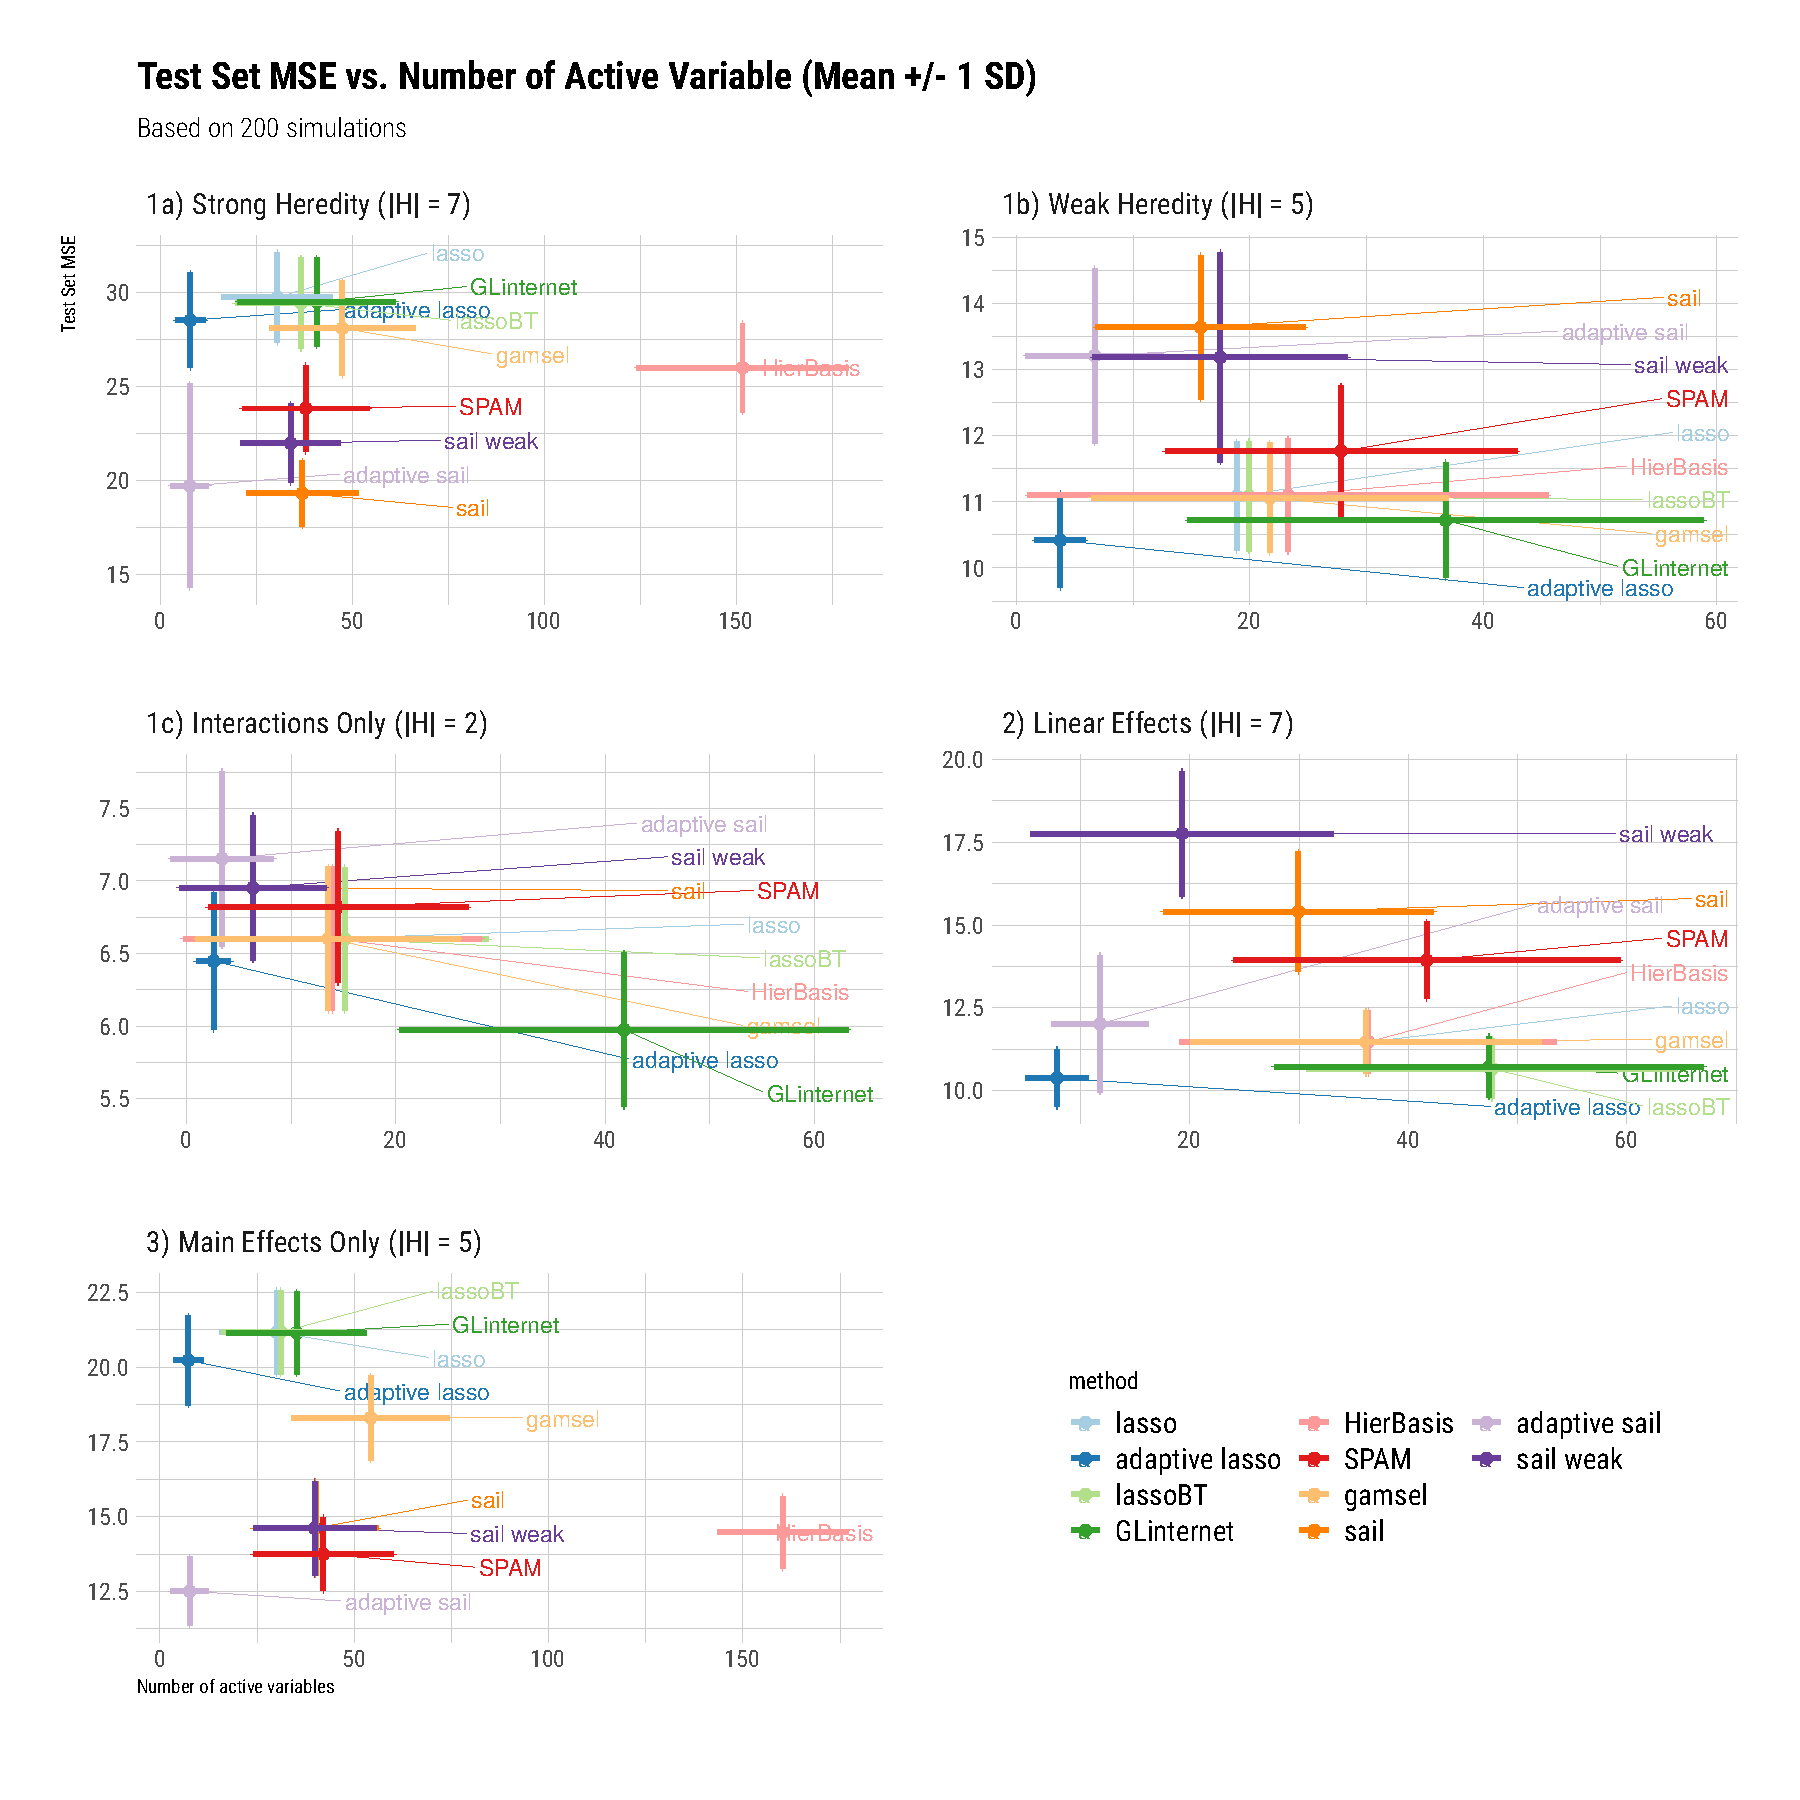
\includegraphics[width=1\linewidth]{figure/plot-mse-nactive-sim-1} 

}

\caption[Test set MSE vs number of active variables results]{Test set MSE vs number of active variables results.}\label{fig:plot-mse-nactive-sim}
\end{figure}


\end{knitrout}


\begin{knitrout}\scriptsize
\definecolor{shadecolor}{rgb}{0.969, 0.969, 0.969}\color{fgcolor}\begin{figure}[H]

{\centering 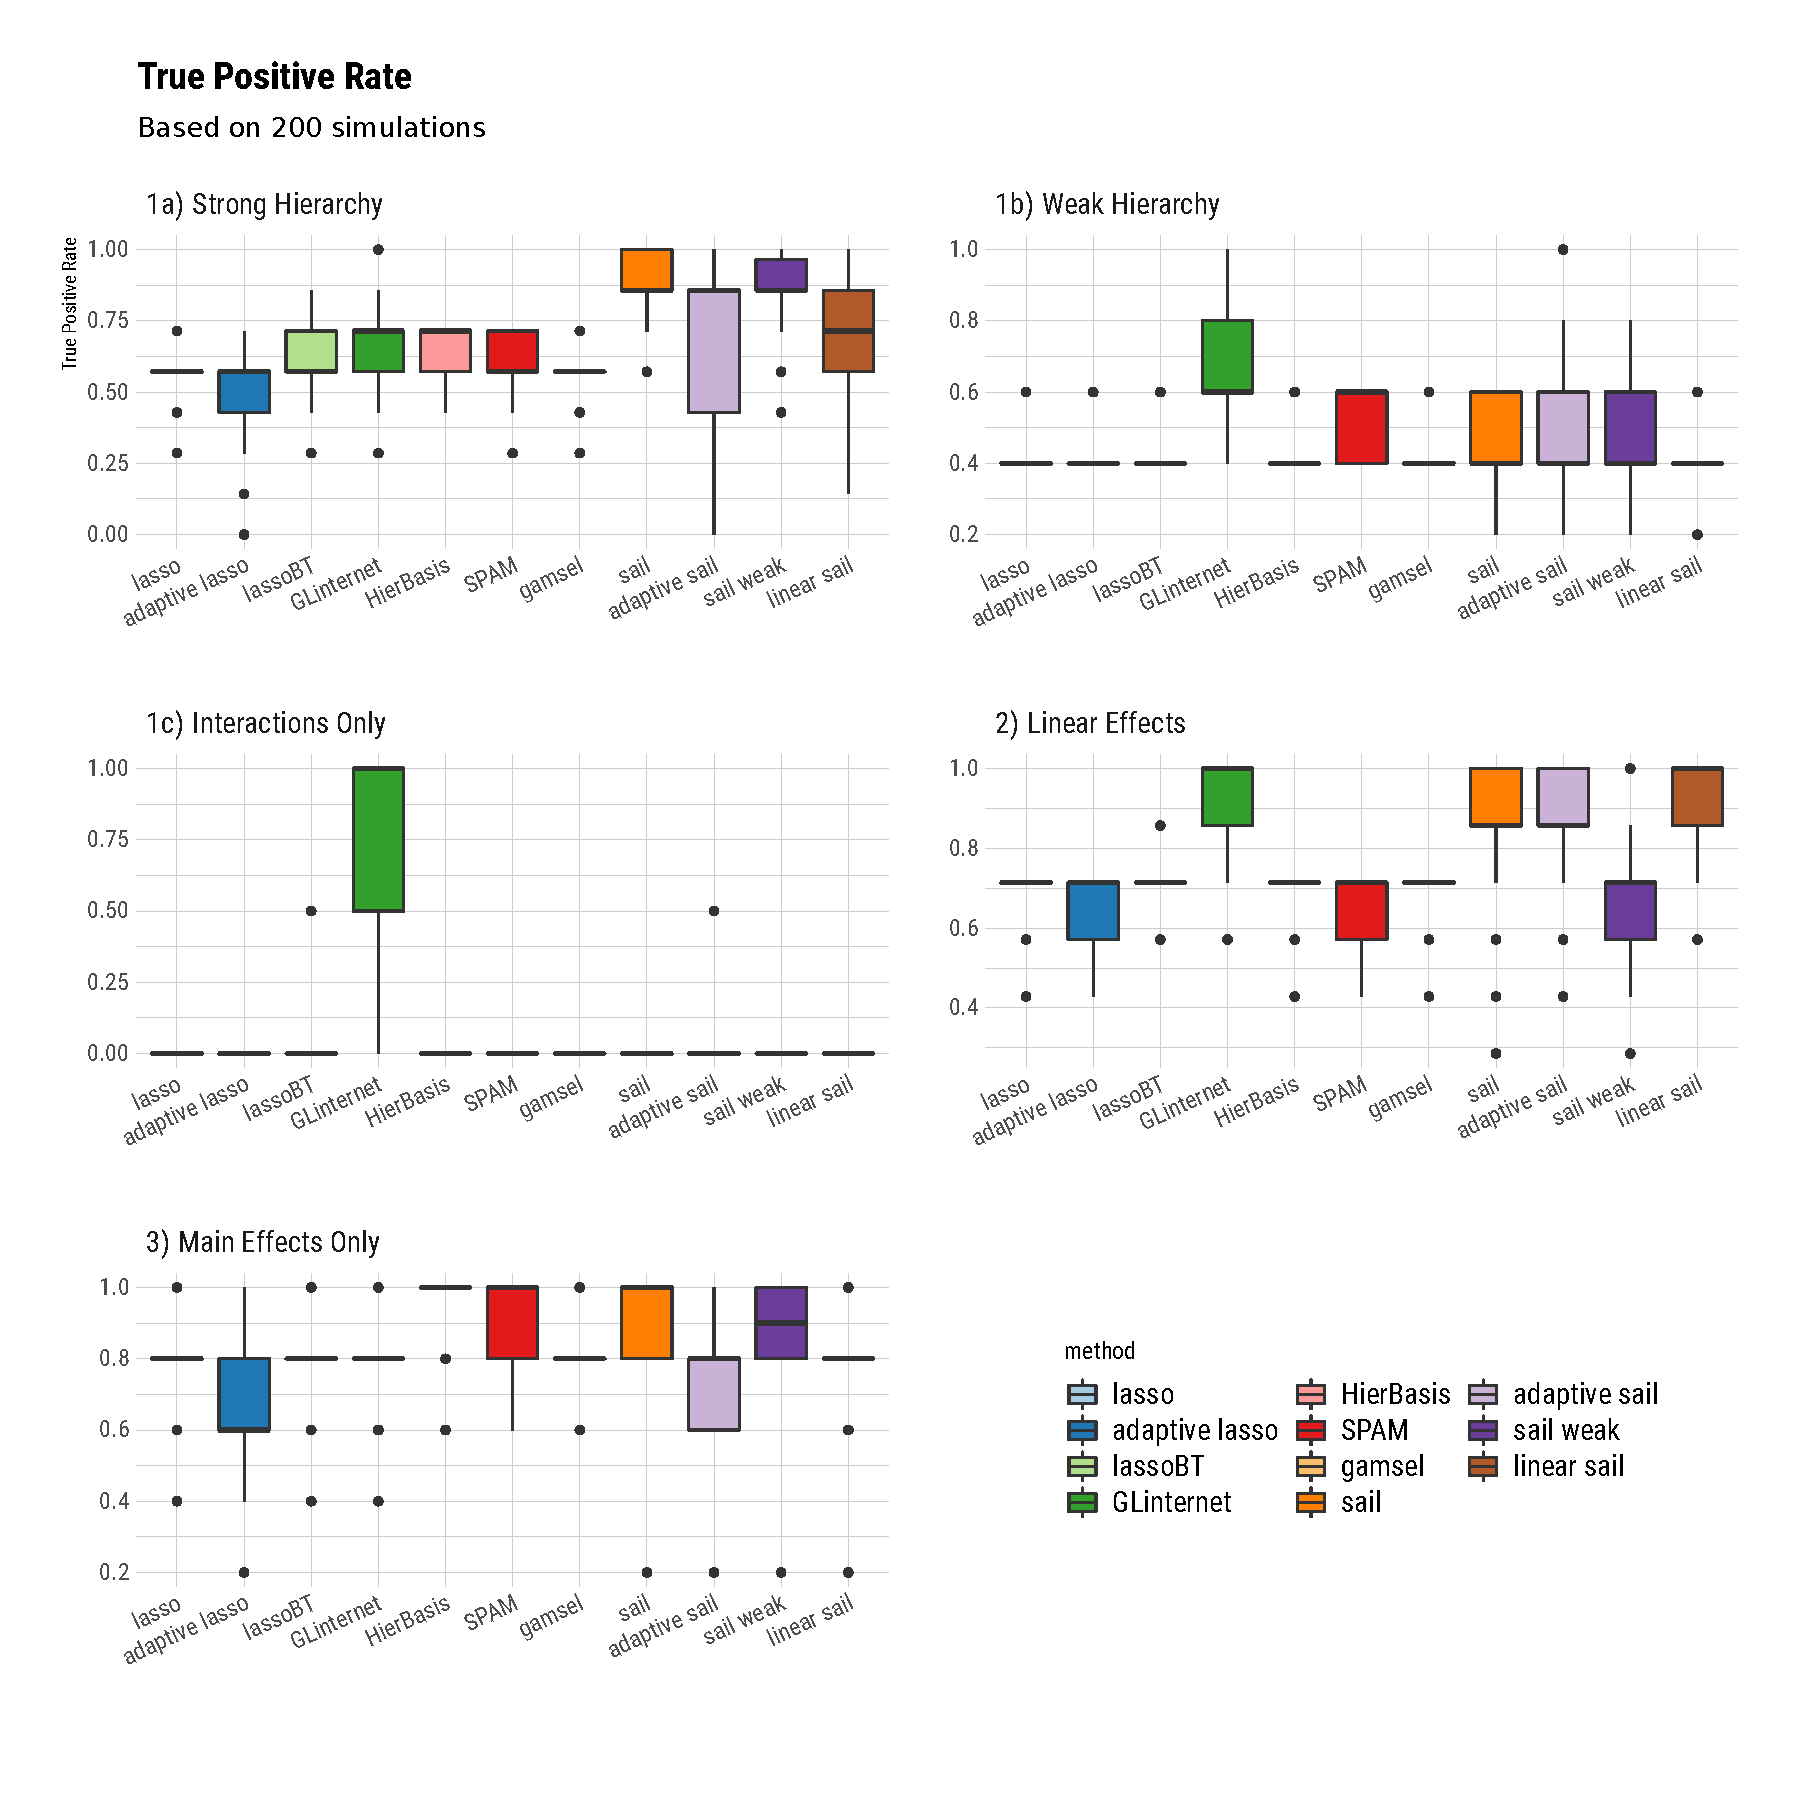
\includegraphics[width=1\linewidth]{figure/plot-tpr-sim-1} 

}

\caption[True positive rate results]{True positive rate results.}\label{fig:plot-tpr-sim}
\end{figure}


\end{knitrout}

\begin{knitrout}\scriptsize
\definecolor{shadecolor}{rgb}{0.969, 0.969, 0.969}\color{fgcolor}\begin{figure}[H]

{\centering 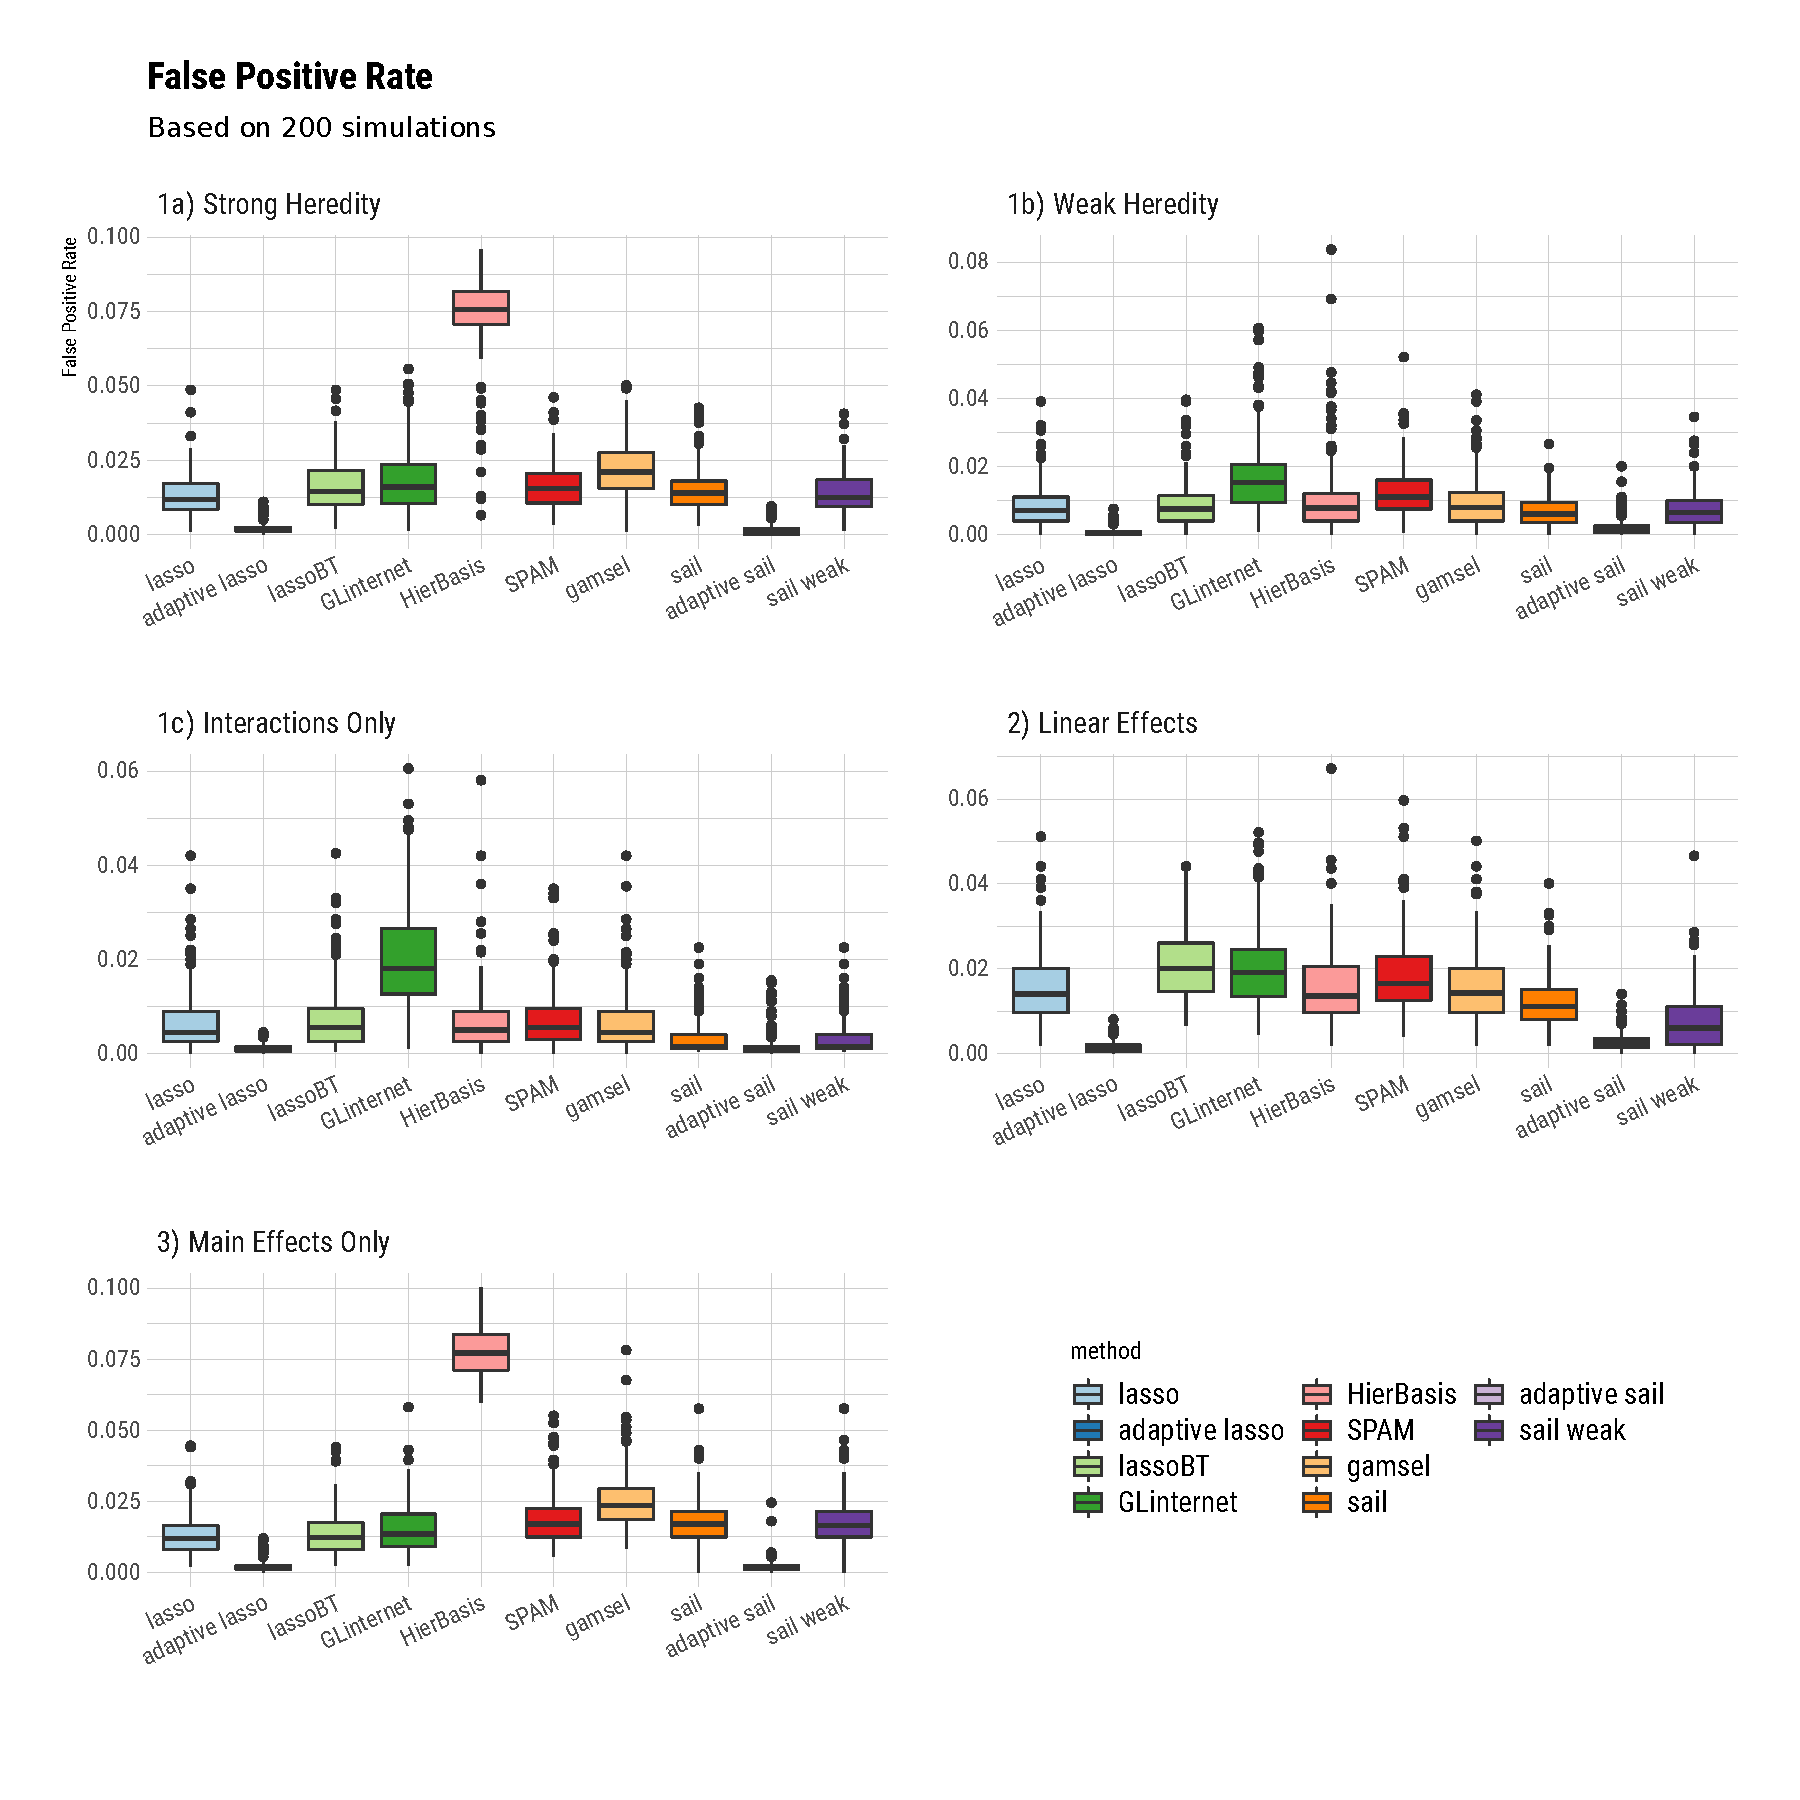
\includegraphics[width=1\linewidth]{figure/plot-fpr-sim-1} 

}

\caption[False positive rate results]{False positive rate results.}\label{fig:plot-fpr-sim}
\end{figure}


\end{knitrout}

\begin{knitrout}\scriptsize
\definecolor{shadecolor}{rgb}{0.969, 0.969, 0.969}\color{fgcolor}\begin{figure}[H]

{\centering 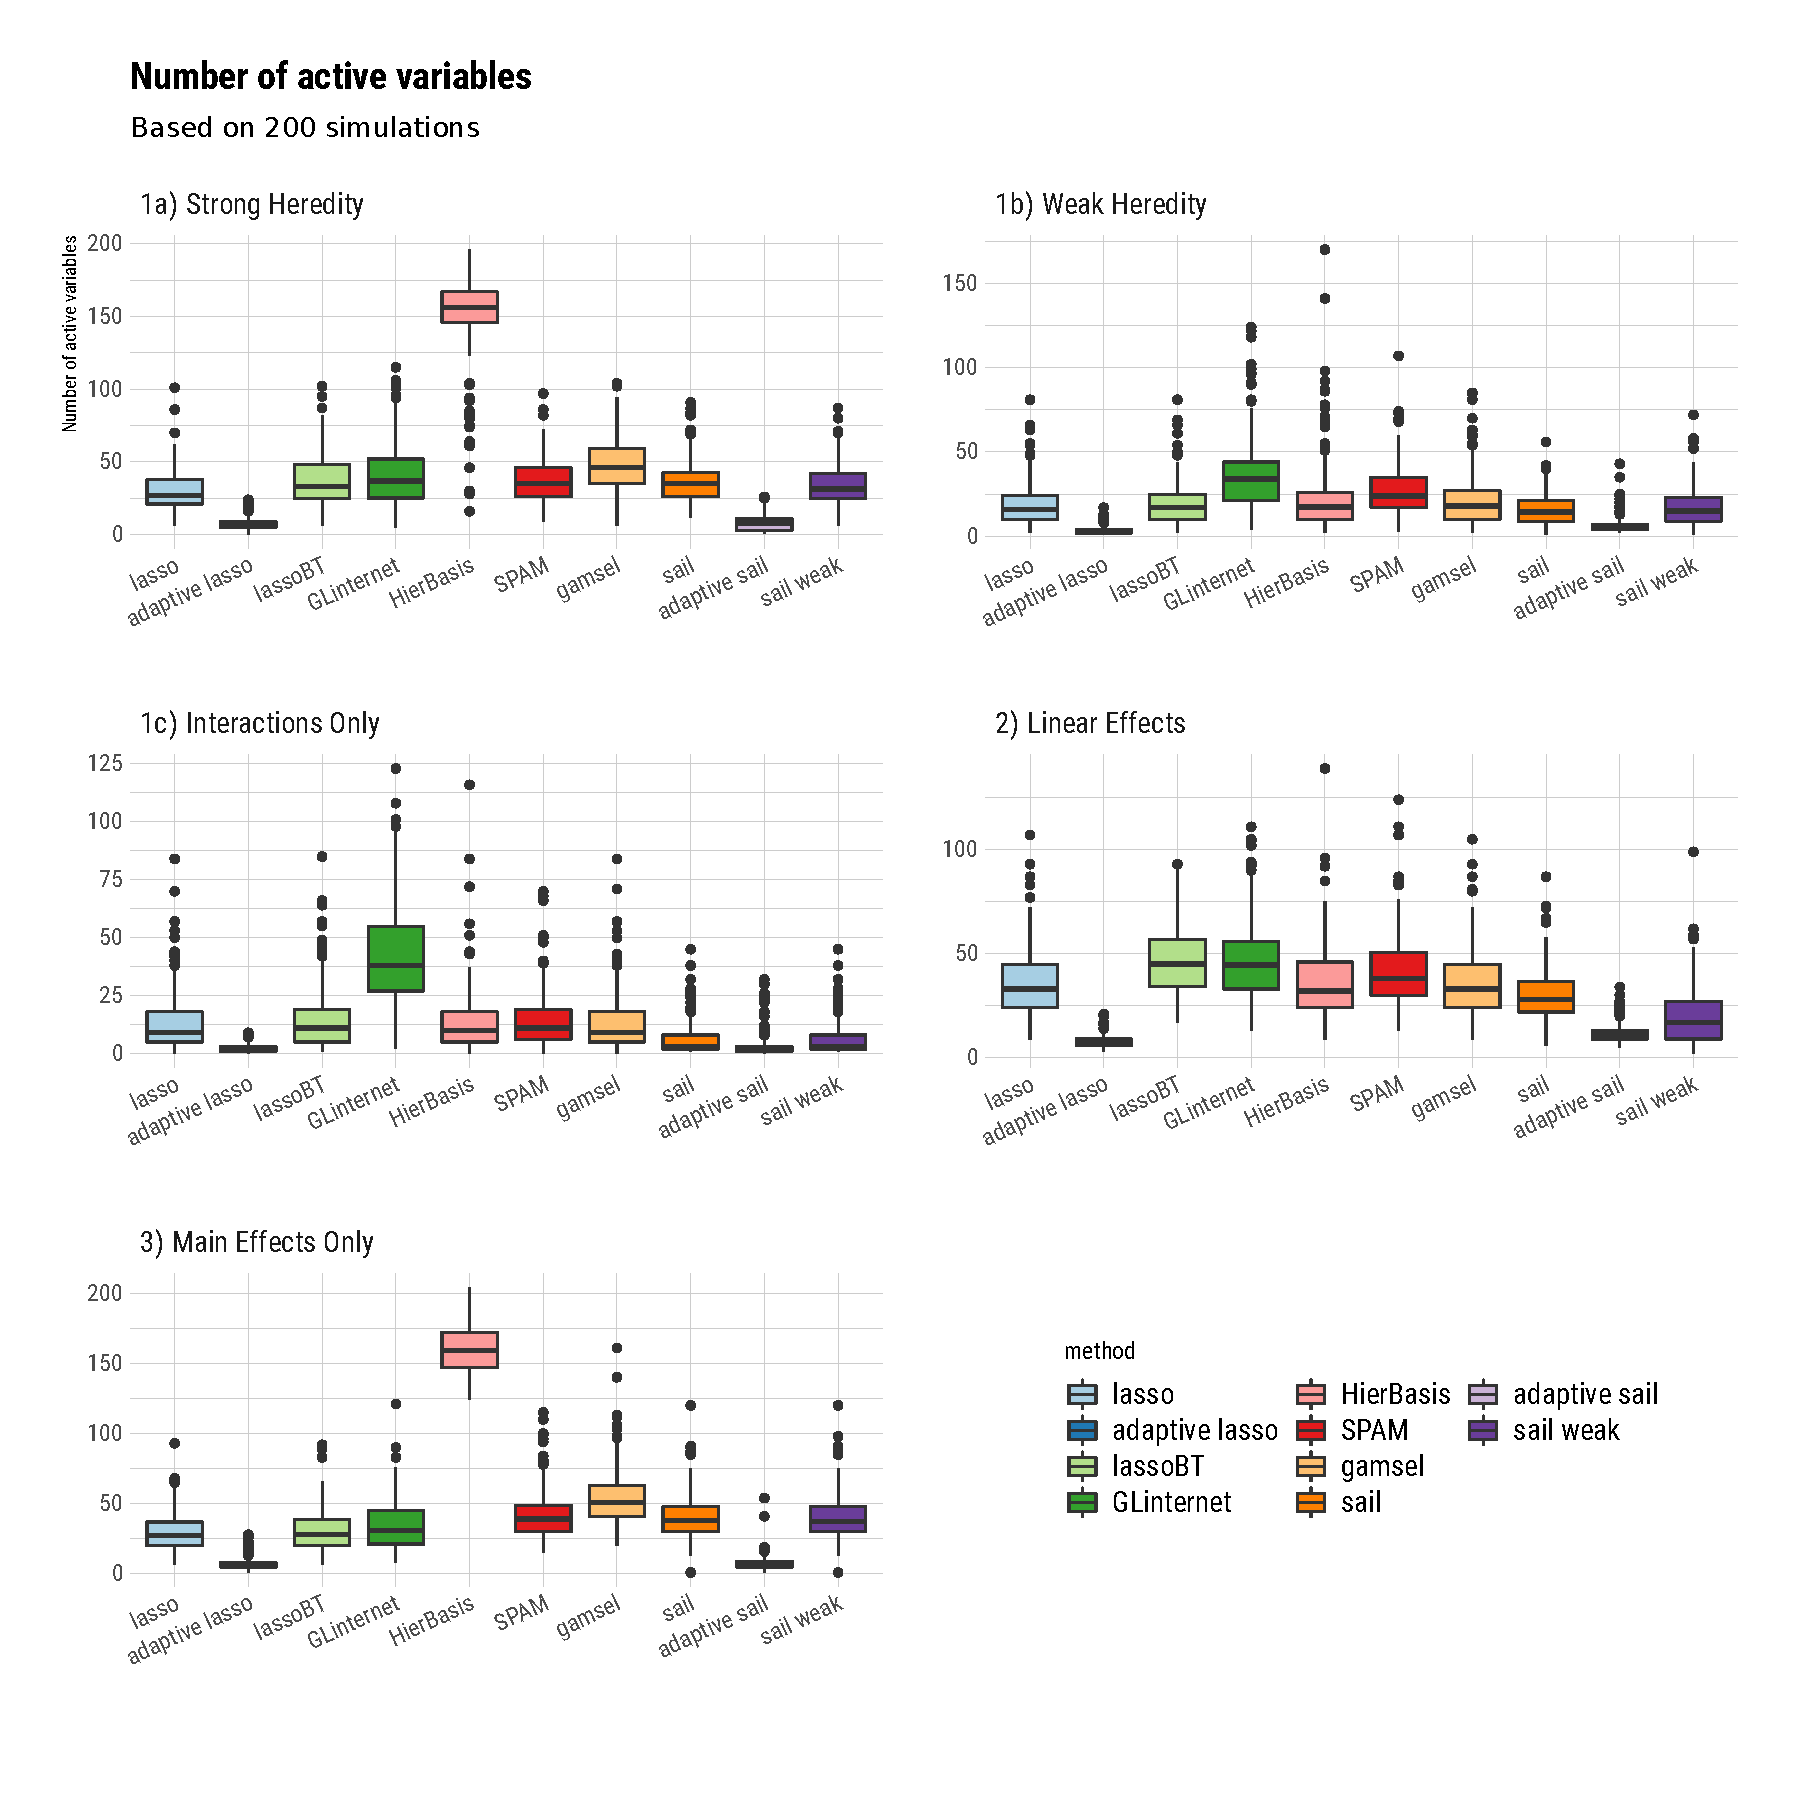
\includegraphics[width=1\linewidth]{figure/plot-nactive-sim-1} 

}

\caption[Number of active variables results]{Number of active variables results.}\label{fig:plot-nactive-sim}
\end{figure}


\end{knitrout}


\begin{figure}[H]
\centering
\includegraphics[scale=0.61]{/home/sahir/git_repositories/sail/my_sims/figures/upset_selection_sail_paramIndex1-2-2.pdf}
\caption{Selection rates across 200 simulations of scenario 1a) for strong heredity \sail.}\label{fig:upset}
\end{figure}





\end{comment}

\FloatBarrier

\section{Additional Simulation Results} \label{ap:sims}

We visually inspected whether our method could correctly capture the shape of the association between the predictors and the response for both main and interaction effects. To do so, we plotted the true and predicted curves for scenario 1a) only. Figure~\ref{fig:main_eff} shows each of the four main effects with the estimated curves from each of the 200 simulations along with the true curve. We can see the effect of the penalty on the parameters, i.e., decreasing prediction variance at the cost of increased bias. This is particularly well illustrated in the bottom right panel where \sail ~smooths out the very wiggly component function $f_4(x)$. Nevertheless, the primary shapes are clearly being captured.

To visualize the estimated interaction effects, we ordered the 200 simulation runs by the Euclidean distance between the estimated and true regression functions. Following Radchenko et al.~\citep{radchenko2010variable}, we then identified the 25th, 50th, and 75th best simulations and plotted, in Figures~\ref{fig:X3} and~\ref{fig:X4}, the interaction effects of $X_E$ with $f_3(X_3)$ and $f_4(X_4)$, respectively. We see that \sail ~does a good job at capturing the true interaction surface for $X_E \cdot f_3(X_3)$. Again, the smoothing and shrinkage effect is apparent when looking at the interaction surfaces for $X_E \cdot f_4(X_4)$.

\begin{figure}[H]
	\centering
	\includegraphics[scale=0.61]{/home/sahir/git_repositories/sail/my_sims/figures/sail_main_eff_paramIndex1_200sims.pdf}
	\caption{True and estimated main effect component functions for scenario 1a). The estimated curves represent the results from each one of the 200 simulations conducted.}\label{fig:main_eff}
\end{figure}


\begin{figure}[H]
	\centering
	\subfloat{\includegraphics[width=0.37\linewidth]{/home/sahir/git_repositories/sail/my_sims/figures/sail_intertruth_X3_paramIndex1_200sims.pdf}}
	\subfloat{\includegraphics[width=0.37\linewidth]{/home/sahir/git_repositories/sail/my_sims/figures/sail_inter25_X3_paramIndex1_200sims.pdf}}\quad
	\subfloat{\includegraphics[width=0.37\linewidth]{/home/sahir/git_repositories/sail/my_sims/figures/sail_inter50_X3_paramIndex1_200sims.pdf}}
	\subfloat{\includegraphics[width=0.37\linewidth]{/home/sahir/git_repositories/sail/my_sims/figures/sail_inter75_X3_paramIndex1_200sims.pdf}}
	\caption{True and estimated interaction effects for $X_E \cdot f_3(X_3)$ in simulation scenario 1a).}
	\label{fig:X3}
\end{figure}


\begin{figure}[H]
	\centering
	\subfloat{\includegraphics[width=0.37\linewidth]{/home/sahir/git_repositories/sail/my_sims/figures/sail_intertruth_X4_paramIndex1_200sims.pdf}}
	\subfloat{\includegraphics[width=0.37\linewidth]{/home/sahir/git_repositories/sail/my_sims/figures/sail_inter25_X4_paramIndex1_200sims.pdf}}\quad
	\subfloat{\includegraphics[width=0.37\linewidth]{/home/sahir/git_repositories/sail/my_sims/figures/sail_inter50_X4_paramIndex1_200sims.pdf}}
	\subfloat{\includegraphics[width=0.37\linewidth]{/home/sahir/git_repositories/sail/my_sims/figures/sail_inter75_X4_paramIndex1_200sims.pdf}}
	\caption{True and estimated interaction effects for $X_E \cdot f_4(X_4)$ in simulation scenario 1a).}
	\label{fig:X4}
\end{figure}







\FloatBarrier


\section{Additional Results on PRS for Educational Attainment} \label{ap:prseduc}

\begin{figure}[H]
		
		{\centering 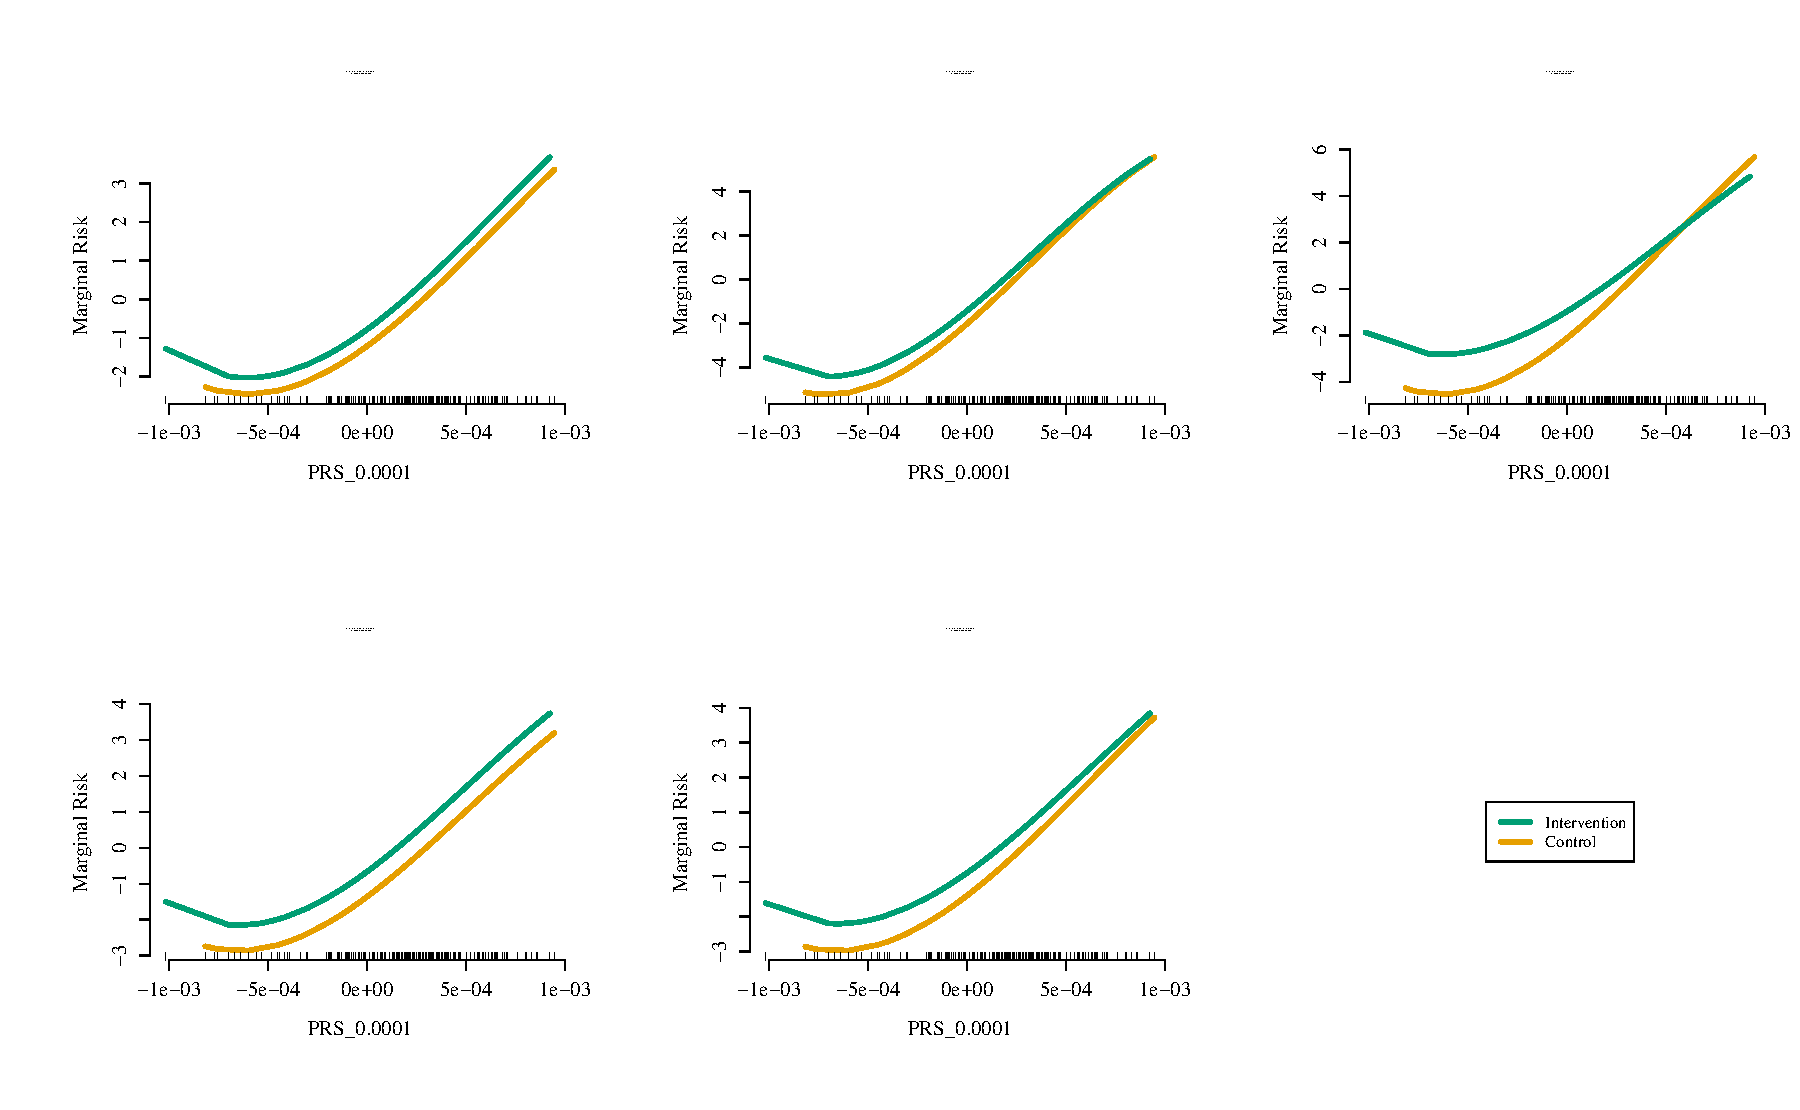
\includegraphics[width=1\linewidth]{../figure/PRS-intervention-interaction-others-1} 
			
		}
		
		\caption{Estimated interaction effect identified by the weak heredity \texttt{sail} using cubic B-splines and $\alpha=0.1$ for the Nurse Family Partnership data for the 5 imputed datasets. Of the 189 subjects, 19 IQ scores were imputed using \texttt{mice}~\citep{buuren2010mice}. The selected model, chosen via 10-fold cross-validation, contained three variables: the main effects for the intervention and the PRS for educational attainment using genetic variants significant at the 0.0001 level, as well as their interaction.}\label{fig:PRS-intervention-interaction-others}
\end{figure}
	
	

\begin{figure}[H]
		
		{\centering 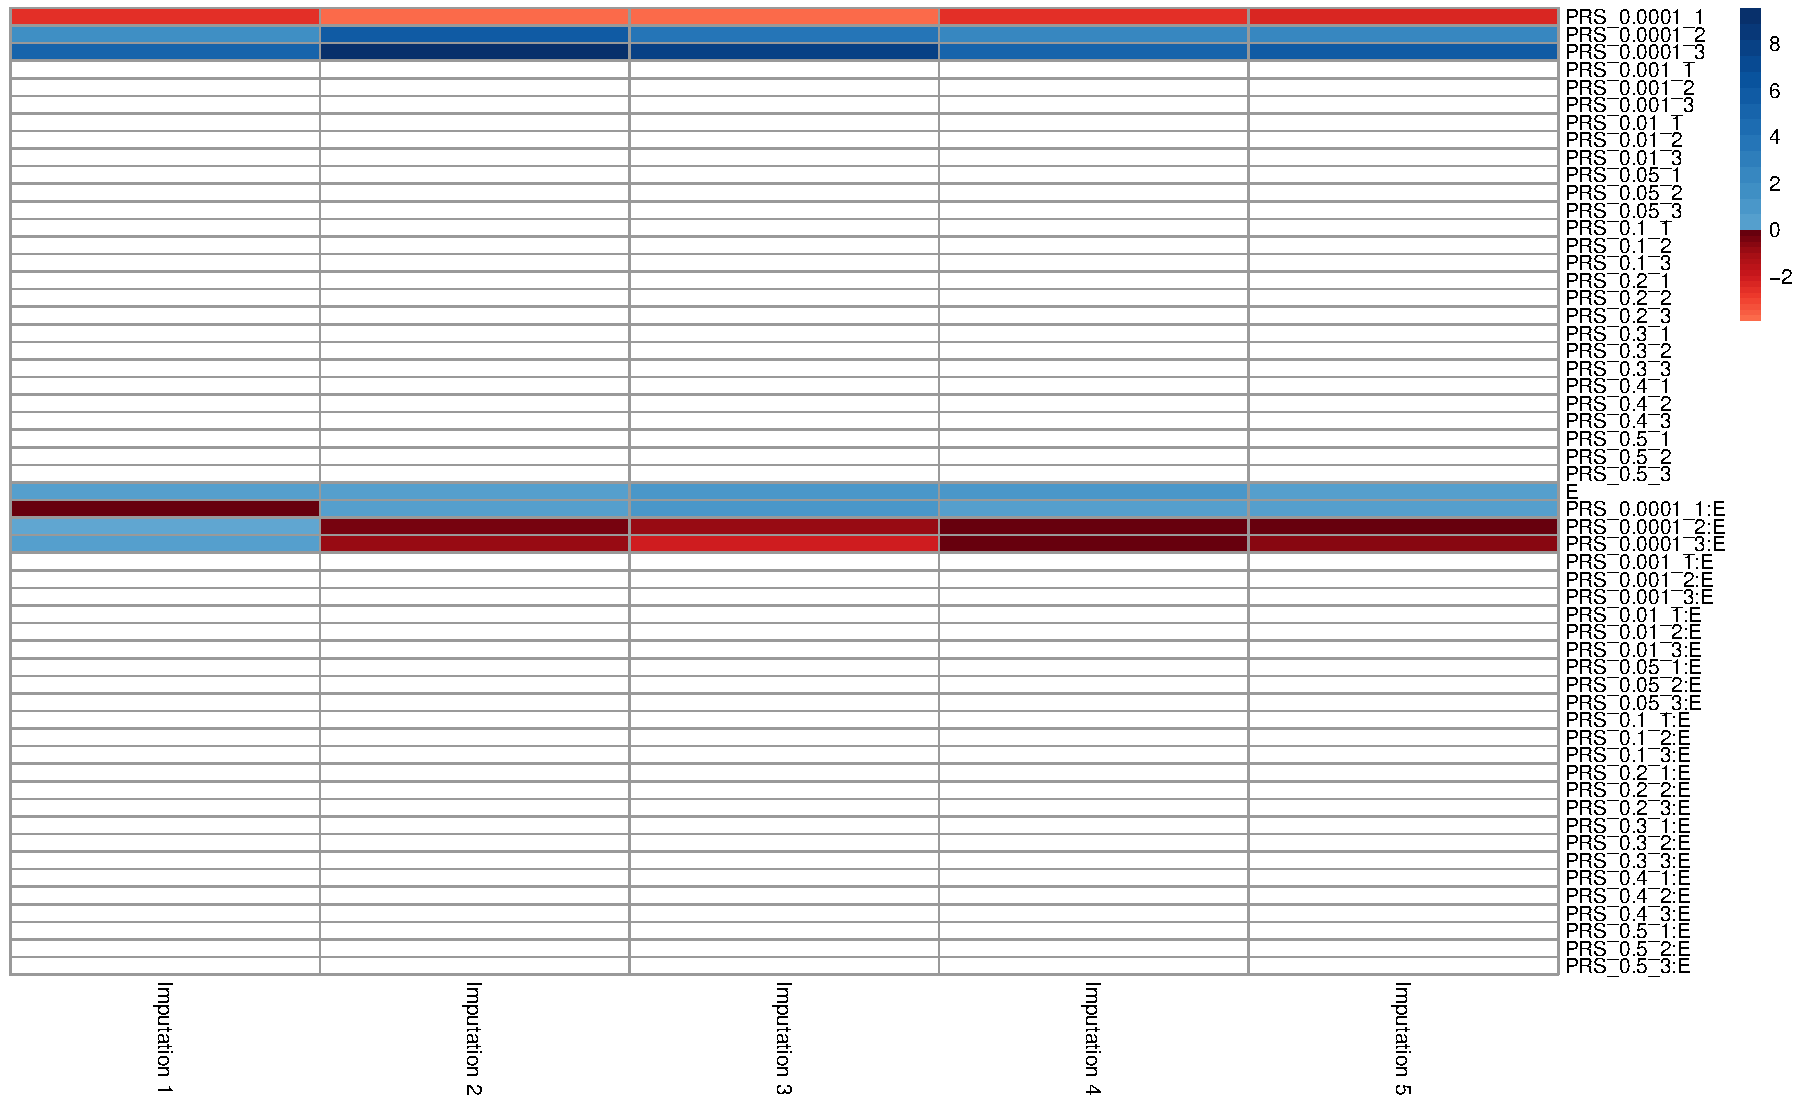
\includegraphics[width=1\linewidth]{../figure/PRS-model-selection-1} 
		}
		
		\caption{Coefficient estimates obtained by the weak heredity \texttt{sail} using cubic B-splines and $\alpha=0.1$ for the Nurse Family Partnership data for the 5 imputed datasets. Of the 189 subjects, 19 IQ scores were imputed using \texttt{mice}~\citep{buuren2010mice}. The selected model, chosen via 10-fold cross-validation, contained three variables: the main effects for the intervention and the PRS for educational attainment using genetic variants significant at the 0.0001 level, as well as their interaction. This results was consistent across all 5 imputed datasets. The white boxes indicate a coefficient estimate of 0.}\label{fig:PRS-model-selection}
	\end{figure}
	

\FloatBarrier


\section{Data Availability and Code to Reproduce Results} \label{ap:rep}

The R scripts used to simulate the data for the simulation studies in Section 4 are provided along with the code for each of the methods being compared. The data used for the two real data analyses in Section 5 are publicly available. The first dataset from the Nurse Family Partnership program is provided by one of the authors of the manuscript (David Olds). The second dataset from the Study to Understand Prognoses Preferences Outcomes and Risks of Treatment (SUPPORT) is publicly available from the Vanderbilt University Department of Biostatistics website. 

\subsection{Datasets}

The datasets are available at \url{https://github.com/sahirbhatnagar/sail/tree/jasa/manuscript/raw_data}


\begin{enumerate}
	\item Nurse Family Partnership program data consists of three files. They are merged together using the script \url{https://github.com/sahirbhatnagar/sail/blob/jasa/manuscript/bin/PRS_bootstrap.R}
	\begin{itemize}
		\item \detokenize{Gen_3PC_scores.txt}
		\item \detokenize{IQ_and_mental_development_variables_for_Sahir_with_study_ID.txt}
		\item \tiny \detokenize{NFP_170614_INFO08_nodup_hard09_noambi_GWAS_EduYears_Pooled_beta_withaf_5000pruned_noambi_16Jan2018.score}
	\end{itemize}
	\normalsize
	\item The SUPPORT data consists of a single file:
	\begin{itemize}
		\item \url{https://github.com/sahirbhatnagar/sail/blob/jasa/manuscript/raw_data/support2.csv}
	\end{itemize}
\end{enumerate}

All datasets are in \texttt{.txt} format. Code used to read in the datasets are provided in the section below. All output from this project published online is available according to the conditions of the Creative Commons License (\url{https://creativecommons.org/licenses/by-nc-sa/2.0/})

\subsection{Code}

The software which implements our algorithm is available in an R package published on CRAN (\url{https://cran.r-project.org/package=sail}) version 0.1.0 with MIT license. The paper itself is written in knitr format, and therefore includes both the code and text in the same \texttt{.Rnw} file. 

The scripts and data used to produce the results in the manuscript are available at \url{https://github.com/sahirbhatnagar/sail/tree/jasa/manuscript}. %This is the jasa branch with commit number 7be7ecd1b5404796a88936026bf680a7e2529798. 

The knitr file which contains both the main text and code is available at: \url{https://github.com/sahirbhatnagar/sail/blob/jasa/manuscript/source/sail_manuscript_v2.Rnw}

The manuscript was compiled using R version 3.6.1 with knitr version 1.25.

The bootstrap analysis was run in parallel on a compute cluster with 40 cores. Though this is not necessary to reproduce the results, it definitely speeds up the computation time.  

\subsubsection{Instructions for Use}

All tables and figures from the paper can be reproduced by compiling the knitr file. The easiest way to reproduce the results is to download the GitHub repository and compile the knitr file from within an R session as follows:

\begin{enumerate}
	\item Download the GitHub repository \url{https://github.com/sahirbhatnagar/sail/archive/jasa.zip}
	\item From within an R session, run the command: \texttt{knitr::knit2pdf('sail\_manuscript\_v2.Rnw')}
\end{enumerate}

Note that to speed up compilation time, we have saved the simulation and bootstrap results in \texttt{.RData} files available at \url{https://github.com/sahirbhatnagar/sail/tree/jasa/manuscript/results}. These \texttt{.RData} files are called directly by the knitr file. 

Note also that the R scripts used to generate the results are called from the knitr file using the `code externalization' functionality of knitr (\url{https://yihui.org/knitr/demo/externalization/}). That is, the actual R code is stored in R scripts and not within the knitr file. These R scripts are available at \url{https://github.com/sahirbhatnagar/sail/tree/jasa/manuscript/bin}. 

The expected run time to compile the manuscript is about 5 minutes on a standard desktop machine, assuming that you are using the pre-run simulation and bootstrap results. 

\subsubsection{R Package Vignette}
A website with two vignettes has been created for our sail package available at \url{https://sahirbhatnagar.com/sail/}

The 2 vignettes are:

\begin{enumerate}
	\item \url{https://sahirbhatnagar.com/sail/articles/introduction-to-sail.html}
	\item \url{https://sahirbhatnagar.com/sail/articles/user-defined-design.html}
\end{enumerate}


\bibliographystyle{biom} \bibliography{GEbib}

\end{document}






